%*****************************************
\chapter{Inflammation}
\label{ch:inflammation}
%*****************************************

%*****************************************
\section{Introduction}
%*****************************************

Inflammation has been a well-known condition to mankind since the first time a caveman kicked a rock too hard, and everyone reading this text has experience inflammation in their life. Text from ancient Egyptians used frankincense and myrrh to reduce pain and swelling \cite{Kadioglu2016}. Hippocrates was the first to describe using the word οἴδημα ( /oídēma/, edema) and identify it as an important component of the healing process \cite{Touwaide1999}. In the modern era, the discovery of anti-inflammatory drugs like aspirin and corticosteroids in the 20th century revolutionized the treatment of inflammatory conditions. \cite{Granger2010}

% (maybe add here a paragraph about what are the modern drug targets and genetics and so on)

Inflammation has 4 main characteristics: heat, pain, redness, and swelling. The combination of these may lead to a 5th one which is loss of function in the affected area. The nature of each of these conditions will be revealed throughout this chapter. Inflammation is a natural process that the body uses to fight infections and eliminate the cause of inflammation, clear out the area of elements that shouldn't be there, and repair the tissue if damaged. Similar to fever, it has a bad name with the general population even for mild cases despite being a beneficial and necessary process for recovery. People tend to self-medicate in excess with antipyretics and anti-inflammatories which is counterproductive for both healing processes \cite{Serhan2014}. This process of acute inflammation is inherent to the natural healing process of an organism and overall, the natural pathways of inflammation do not pose a risk to the organism's life, and it is counterproductive to interfere with it, as such interference may ultimately impair the healing process in the long run. On the other hand, autoimmune reactions and chronic inflammations are the undesirable form of inflammation that may lead to lasting damage; often in the form of scar tissue.

At the end of this chapter (section \ref{ref:onlinkPanel}) I discuss the 92 different inflammatory biomarkers upon which the social influence in the inflammation article is founded. However, comprehension of these biomarkers is a complex subject and requires an elaborate introduction to the intricacies of the inflammatory processes. Half of the Inflammation chapter aims to aid the understanding the background of how these 92 biomarkers work. It also serves as a base to further understand the immunoevasion properties of \textit{S. Aureus}, and homeostatic properties of vitamin D. Anyone familiar with immunology should be able to skip directly to section \ref{in:cycle}.

%*****************************************
\section{Immunology basic concepts}
%*****************************************

This section serves as an introduction of basic and easy concepts related to immunity.

\subsection{Reactive Oxygen Species}

\gls{ros} are a natural by-product of cellular metabolism and immune system responses which the influence of heavy metals, tobacco, radiation, or microplastics can overproduce. Excess amounts of ROS damage DNA, lipids, and proteins. This is bad for cells, but good if those cells are bacteria or viruses that we want to destroy.

\subsection{Extracellular matrix}

The extracellular matrix is the material that fills the spaces between cells in tissues and provides the structural support that allows tissues to maintain their shape and function properly. During inflammation, fibroblasts play an important role in the repair and remodeling of damaged tissues. They are activated by cytokines and growth factors that are released by immune cells. As a results they fill the extracellular matrix with collagen, elastin, and fibronectin, which translate into tissue healing.

\subsection{Antigens}

\gls{ag} can be proteins, peptides, polysaccharides, lipids, or nucleic acids. Antigens can be parts of a normal functioning cell or part of a foreign pathogen or substance. They serve as an identification card of whatever cell is holding the Ag.

\subsection{Major Histocompatibility Complex}

The \gls{mhc} proteins are found on the surface of almost all cells with nuclei in the body. They catch antigens inside the cell and present them to the outside. There are three types of MHC, and overall the main difference is what type of leukocytes or complement protein they interact with.

\subsection{Antigen presenting cells}

And \gls{apc} is a leukocyte that can present foreign pathogens or abnormal tumorous cells antigens to other cells of the immune system. The professional APCs are dendritic cells, macrophages, and B-cells. Besides those, any other cell in the body that has a nucleus also has an MHC, and can also be an APC, but these are called non-professional.

\subsection{CD proteins}

The \gls{cd} is a protocol used to identify cell surface molecules. There are 371 known CD molecules in humans. Generally, they play a role in cell signaling. Two important CD proteins are:

\begin{itemize}
\label{inf:cd4cdprotein}

    \item{\textbf{CD4 protein}} is a co-receptor for the \gls{tcr} on T-helper cells, helping to enhance the binding and sensitivity of the \gls{tcr} to antigen-MHC2 complexes. This is the primary receptor for the \gls{hiv}, which is why this virus targets immune cells leading to immunodeficiency. Other cells such as monocytes and dendritic cells can also express CD4. Any cell that expresses CD4 on the surface is known as a CD4+ cell.

    \item{\textbf{CD8 protein}} is another TCR that binds to antigen-MHC1 complexes. Is mostly expressed on cytotoxic T cells but can also be found on natural killer cells and dendritic cells. Any cell that expresses CD8 on the surface is known as a CD8+ cell.
    
\end{itemize}

\subsection{Cytokines}
\label{ref:inflammationCytokines}

Cytokines are a group of small signaling molecules that coordinate various processes in the human body, such as  immune response activation, changing the states in the inflammation cycle, and the formation of new blood cells (hematopoiesis). They are produced by both immune and non-immune cells. The major groups of cytokines are:

\subsubsection{Chemokines}

    A family of chemotaxis cytokines secreted by cells to make leukocytes move in a particular direction, hence the name "kino" (movement). They are classified according to their behavior and protein structure. For example, a "C-C motif" just makes reference to the type of structure in which it has two adjacent cysteines. A "C-X-C motif" is the same, but in between cysteines there is another amino acid, hence the X. "Chemotaxis" means that it allows for movement, while "chemotactic" refers to how good or bad a particular protein does so.

\subsubsection{Growth factors}
\label{in:GF}

    These cytokines are involved in regulating cell growth, proliferation, and differentiation.

    In particular, we will be interested in \gls{fgf}, a family of cell signaling proteins produced by macrophages. Their function is to regulate normal cell development in animals.

\subsubsection{Interferons}

    Alert other non-immune cells about ready their defenses because the infection is happening and tell immune-cell to come and kill infected cells. They are explained in section \ref{in:inter}

\subsubsection{Interleukins}

    Are the internet of leukocytes and will be explained in section \ref{in:interleukins}.

\subsubsection{Tumor necrosis factors}

    Are both pro-inflammatory and anti-inflammatory signals needed in each stage of inflammation and will be explained in section \ref{in:tnf}    

\subsection{Types of immune responses}

\subsubsection{Humoral vs Cell-mediated}

A humoral immune response works against extracellular pathogens, while a cell-mediated response works against intracellular pathogens and abnormal cells. As a general rule, killing your own cells is a very bad idea that leads to many unwanted problems, and the least preferred type of immune reaction. Therefore, there are a lot of efforts promoting behaviors and diets that promote humoral response and are able to kill the pathogens before they can infect host cells, or to prevent cancer grow.



\subsubsection{Innate vs Adaptive}
\label{in:InnVSAdap}

Overall, innate immunity provides quick but weak protection against a wide range of pathogens. While adaptive immunity takes more time to activate but is more efficient against each specific type of pathogen and provides long-term protection. The function of cells named in this section will be introduced formally in section \ref{in:leukocytes}.

Innate immunity is present from birth (hence the name) and involves physical and chemical barriers that prevent pathogens from entering the body, such as skin, mucous membranes, and stomach acid. Innate immunity also includes cells such as natural killer cells, neutrophils, and macrophages that can recognize and attack foreign invaders, as well as the complement system, which can activate a series of proteins to help identify and destroy pathogens.

Adaptive immunity, on the other hand, is a specific, second line of defense that develops over time as the immune system gains experience and adapts to specific pathogens. This type of immunity involves the production of antibodies which lock to the pathogen's antigens. The first time a pathogen enters the body, neither the antibodies not the cells manufacturing them exist, and it takes a long time, usually around 2 to 3 weeks, for the immune system to mount an effective response. Later on in life, once the pathogen enters the body again, such antibodies are ready to use and the response is shortened to about 2 to 3 days.

\subsection{NF-κB}
\label{inf:nfkb}

\gls{nfkb}, is a collection of proteins that controls the transcription of DNA. In our context, it regulates both the innate and adaptive immune response \cite{Smith2006}. NF-κB can be up or down-regulated by other mechanisms discussed later in this document, and by extension controlling immune reaction. It does it by promoting TNFA, IL1B, and IL18.


\subsection{Homeostasis}

The immune system must be balanced between slacking off and letting foreign agents invade and destroy the body, and being overactive and being the immune system itself the one that destroys the body. Proper functioning of the immune system requires a delicate balance between activation and regulation. This balance is known as immune system homeostasis. Overall, this work falls on the T cells, by maintaining the appropriate levels of cytokines, which maintain the appropriate levels of everything else.

This is also important during inflammation episodes. There are parts of the immune system that are pro-inflammatory and parts that are anti-inflammatory. Both have their roles and both are needed for a successful resolution of an inflammation process, and the existence of neither of them is necessarily good or bad. Their presence is welcome within the time frame in which they are needed, and no more.

\subsection{Leukocytes}
\label{in:leukocytes}

Leukocytes, also known as white blood cells, are a type of immune cell that helps protect the body against infections and diseases. There are several classifications which will be mention in this section to avoid confusion, but in our context we care the most on whether they are granulocytes or not.

Neutrophils, Eosinophils, Basophils, Mast cells, a type of leukocytes that contain granules and are classified as granulocytes. Granules are essentially a bunch of sacks in the cytoplasm organ that release cytokines and will be discussed later with more detail in section \ref{inf:granules}. They are also known as polymorphonuclear leukocytes (PMN) as they have several nuclei. However, neutrophils are the most abundant of these types and they are also referred as PMN despise sharing the group with other leukocytes.

    \begin{figure}[h!]
        \centering
            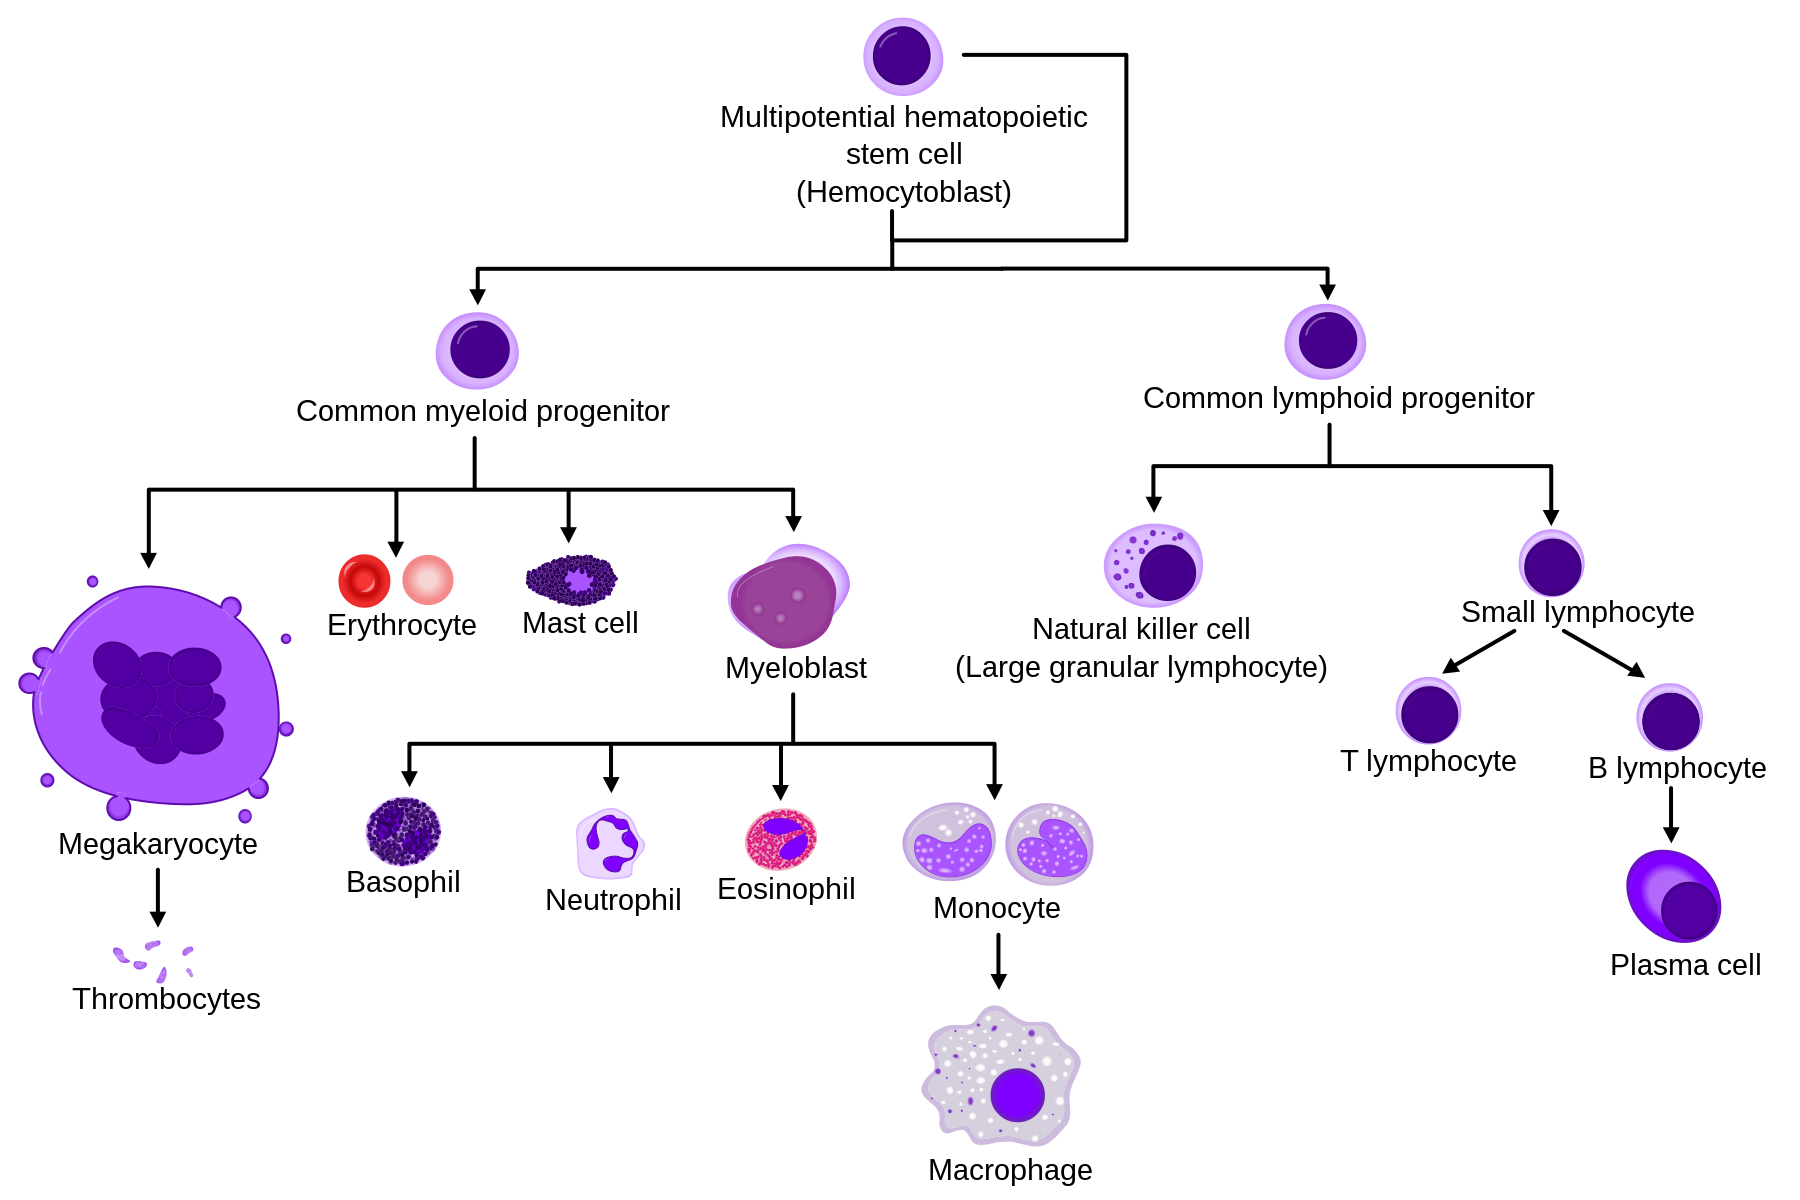
\includegraphics[width=0.7\linewidth]{figures/Inflammation/Hematopoiesis_simple.svg.png} 
        \caption{Overview of the formation of blood cellular components (haematopoiesis). All cellular blood components are derived from pluripotent stem cell root. Image from \href{https://en.wikipedia.org/wiki/File:Hematopoiesis_simple.svg}{Wikimedia}.
        \label{figure:bloodformation}}
    \end{figure}  

Natural killer cells are known large granular lymphocytes (LGL). They also have granules in their cytoplams, but they are not considered to be granulocytes. They have a different root of pluripotent differentiation (figure \ref{figure:bloodformation}), and as such their granules have different functions related to direct killing rather than helping the immune system.

Monocytes develops from the same stem root, and while they occasionally display another type of granule (azurophilic granule), are not classified as granulocytes either. They also have only one nucleus but it shaped is elongated and indented, which might be confused with having several nuclei.

\subsubsection{Neutrophils}

These are the most abundant and are responsible for the phagocytosis of bacteria and other foreign substances. They have a similar role as macrophages, but neutrophils are the first to act and are not professional APCs. They are found in the blood from where they migrate to inflammation sites through a process known as chemotaxis. This involves the detection of a chemical signal (chemoattractant) released by cells at the site of infection. The neutrophil follows the gradient of the chemoattractant until it reaches the site of infection.

\subsubsection{Eosinophils}

They play a role in the body's immune response to parasitic infections, allergies, and asthma. They contain granular structures which are bright red dyed with eosin, hence the name. High levels are correlated with eosinophilic asthma and hypereosinophilic syndrome.

\subsubsection{Basophils}

Basophils are responsible for releasing histamine and other inflammatory molecules in response to allergens, parasites, and other types of foreign substances. Basophils make up less than 1\% of all white blood cells in the body.
        
\subsubsection{Mast cells}

Another type of leukocyte which are found throughout the body, particularly in tissues that are in contact with the external environment like the skin, lungs, and digestive tract. They are involved in the regulation of the immune system. When they are overactive, they can upregulate the immune system too much causing allergies, asthma, and autoimmune disorders.

\subsubsection{Monocytes}

    Monocytes are the largest type of white blood cell and play a role in the phagocytosis of foreign substances. Alongside neutrophils, they belong to the phagocytes group. Monocytes are further subclassified as:

    \begin{itemize}
        
        \item{\textbf{Macrophages}} are large white blood cells that are primarily responsible for phagocytosis. Macrophages also play a key role in presenting antigens to other cells of the immune system, which enables them to launch an appropriate immune response. They are mostly concentrated in the spleen, liver, and lymph nodes. When the proper signaling arrives, they migrate to blood vessels and from there to the inflammation site. Macrophages are further divided into two types:

            \begin{itemize}

                \item{\textbf{M1}} are activated by pro-inflammatory cytokines or \gls{lps}. They produce pro-inflammatory cytokines themselves and kill microbes by phagocytosis or ROS-like substances.
                
                \item{\textbf{M2}} are activated by anti-inflammatory cytokines. These macrophages collaborate in tissue repair.

            \end{itemize}
            
        \item{\textbf{Dendritic cells}} are specialized immune cells that are found primarily in tissues that are in contacts with the external environment, such as the skin, lungs, and intestines. Dendritic cells are known for their ability to capture and process antigens, which they then present to other immune cells in order to activate an immune response. Dendritic cells are particularly important in the initiation of adaptive immune responses,

    \end{itemize}

\subsubsection{Natural killer cells}

\gls{nk} cells identify and destroy human cells. Typically those cells would be infected or cancerous cells presenting an abnormal antigen in the MCH1. But they can also be healthy cells that lack the proper MHC1, such as in transplants from another body, cancer cells that typically display less MHC1, or simply that NK cells can't recognize MCH1 as self due to an autoimmune disorder. Unlike B and T cells, NK cells do not require prior activation which allows them to act very fast preventing further cancer growth or incubation time. They also produce cytokines that help regulate the immune response. On the downside, they do not have memory or clonal expansion capabilities.

\subsubsection{Lymphocytes}

Lymphocytes are involved in the immune response, producing antibodies against foreign substances and attacking infected or cancerous cells. There are divided into further categories:

    \begin{itemize}

        \item[B-lymphocytes] are involved in producing antibodies that will help other leukocytes to recognize and kill the pathogen, or prevent the pathogen to do its function correctly. The basic sub-classification is:

        \begin{itemize}

            \item{\textbf{B-cells}} are both activated by APC and APC themselves, they can help regulate the activity of T-cells, but this is not their main function. They are responsible for producing antibodies. Antibodies are also known as \gls{ig}, and are sub-classified into the following categories:
    
                \begin{itemize}
        
                    \item{\textbf{IgA:}} Found in high concentration in saliva, tears, breast milk, and mucous membranes.
            
                    \item{\textbf{IgD:}} These antibodies are found on the surface of B cells when they exist in the bone marrow and are co-expressed with IgM. But to this day their function is not fully understood.
            
                    \item{\textbf{IgE:}} Bind to allergens such as pollen, animal dander, and food particles, triggering the release of histamine.
            
                    \item{\textbf{IgG:}} Common in the blood and tissue fluids, they have a role in the adaptative immune response. They are also the only type of antibody that cross the placenta from a mother to the fetus, providing temporary immunity.
            
                    \item{\textbf{IgM:}} First to be produced in response to an infection and are effective against general bacteria and viruses.
                
                \end{itemize}
    
            When a B-cell changes producing one Ig to a different one is known as class switching. Later on, we will also talk about lipid mediator class switching, but despise the name, the two concepts are unrelated.
    
            \item{\textbf{Plasma cells}} Are specialized B-cells that can only generate one type of antibody which is triggered by one particular antigen. They serve as a specialized and quick response in current infections and have a short time lifespan.
        
            \item{\textbf{Memory B cells}} are the same as plasma cells, but they have a long time lifespan and provide long-term immunity for years. When memory B cells finally die, you need a memory shot vaccine for their related disease. They can be activated by the pathogen directly, but is more common that they are awakened by memory T cells.        

        \end{itemize}


        \item {T cells} are involved in killing infected cells and regulating the immune system producing cytokines. They are called "T" because they mature in the thymus, but their further sub-classification and function range widely:

        \begin{figure}[ht]
            \centering
                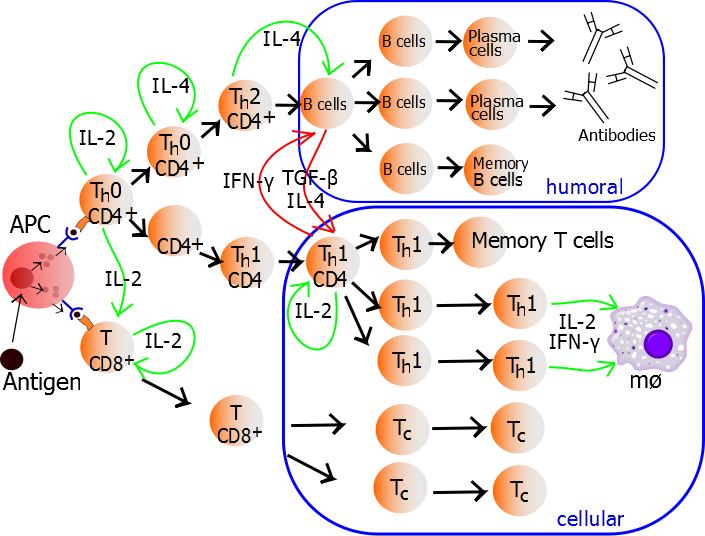
\includegraphics[width=0.5\linewidth]{figures/Inflammation/Lymphocyte_activation.png} 
            \caption{Overview of the T-cells activation and differentiation. Image from \href{https://en.wikiversity.org/wiki/WikiJournal_of_Medicine/Medical_gallery_of_Mikael_H\%C3\%A4ggstr\%C3\%B6m_2014}{"Medical Gallery of Mikael Häggström 2014". WikiJournal of Medicine}}.
            \label{figure:Thell}
        \end{figure}  
    
            \begin{itemize}
    
                \item{\textbf{\gls{th}:}} bind to APC and stimulate the production of antibodies and cytokines. When T-cells are immature they are known as "Th" or "Th0". Then they get activated by APC turning into two main types, "Th1" or "Th2". Th1 cells lead to a cell-mediated response, and Th2 cells lead to a humoral immune response. "Th17" type is a third type that produces IL-17, a pro-inflammatory substance especially good at fighting extracellular pathogens and fungi. THαβ is the fourth type and  provides host immunity against viruses by activating Natural Killer cells. Any Th cell that expresses the CD4 protein, is also known as CD4+ cells.
        
                \item{\textbf{Cytotoxic T cells:}} These cells directly kill infected cells same as NK cells. The cells are known by many other names, including TC, cytotoxic T lymphocyte, CTL, T-killer cell, cytolytic T cell, CD8+ T-cell, and killer T cell, which may cause confusion with other T cell names. Cytotoxic T cells are part of the adaptive immune system and are highly specific in recognizing and attacking infected or abnormal cells that display a specific antigen on their MHC. In contrast, NK cells do not recognize specific antigens, but rather detect and target cells that have decreased expression of normal surface proteins, such as MHC1. Cytotoxic T cells can develop a long-lasting immunological memory after encountering an antigen, allowing for a more rapid and efficient response upon re-exposure.
        
                \item{\textbf{Regulatory T cells:}} These cells help control the immune response by suppressing the activity of other T cells, preventing them from attacking healthy cells.
        
                \item{\textbf{Natural killer T cells:}} Not to be confused with either Cytotoxic T cells (T-killer cells) or Natural Killer cells (NK cells). They can also be CD4+ and CD8+ cells. They recognized microbial lipids and enhance humoral immunity. Upon activation, they produce large quantities of \gls{ifng}, IL-4, and granulocyte-macrophage colony-stimulating factor, IL-2, IL-13, IL-17, IL-21, and \gls{tnfa} among others. Lack of NKT shows autoimmune diseases, autoinflammatory diseases, and cancers.
        
                \item{\textbf{Memory T cells:}} There are 5 types of memory T cells and 3 major ways of activation. They also share some functions with memory B cells. But simplifying their function consists of recognizing previously encounter pathogens and activating the appropriate memory B cells. They actually have a relatively short lifespan and need to be manufactured constantly.
    
            \end{itemize}
        
    \end{itemize}


 

\subsection{Granules}
\label{inf:granules}

Granules are sacs contained in the cytoplasm and contain inflammatory mediators. The two main types of cells that have granules are lymphocytes of the granulocytes class and endothelial cells. In the case of the endothelial cells, granules are stored inside the Weibel–Palade body. Here we list the main inflammatory mediators released from granules during an inflammation process.

\subsubsection{Von Willebrand factor}
\label{in:VonWill}

\gls{vwf} is a protein that plays a key role in the initial stages of clotting by binding to platelets and forming a plug at the site of injury. In an inflammatory process produced by an injury, the most important mechanism is to first stop the bleeding quickly so you don't die. Afterward, other mechanisms will promote vasodilation so the leukocytes can actually go there to do their job. It deficiency might be caused by the most common hereditary blood-clotting disorder in humans \gls{vwd}, which is presented in the form of too much bleeding tendency, such as bruising, nosebleeds, heavy menstrual periods, even severe internal bleeding in the worse cases.

\subsubsection{Selectin}
\label{in:selectin}

Selectins are a family of \gls{cam}. The work of selectin in epithelial cells is slow down leukocyte rolling alongside the interior of blood vessels, and bring it out of the blood vessel so it can go into the source of inflammation and deal with it. There are three subsets:

\begin{itemize}

    \item {\textbf{P-selectin}}. The release of histamine or thrombin in the inflammation sites makes endothelial cells rise P-selectin stored in the cytoplasm up to their cell wall. These are proteins in the shape of "hooks" that catch leucocytes or platelets near the inflammation site.
 
    \item {\textbf{E-selectin}}. Release of IL-1 and TNF-α by macrophages in the inflammation site induces expression of E-selectin on endothelial cells bringing leukocytes inside. They work similarly to P-selectin, but E-selectin takes longer to be activated and is produced and released rather than stored in the cells.
    
    \item {\textbf{L-selectin}} is expressed in leukocytes and they hook to the P/E-selectin expressed in the endothelial cells. L-selectin is also present on the surface of the human embryo and works the same way as with leukocytes facilitating its adhesion to the endometrium.
    
\end{itemize}

\subsubsection{Bradikin}

Bradykinin is a vasodilator, leading to increased blood flow into the affected area. It also increases vascular permeability, allowing inflammatory cells and proteins to move from the bloodstream into the affected tissues. Additionally, bradykinin activates pain receptors, leading to the sensation of pain associated with inflammation.

\subsubsection{Histamine}
\label{in:histamine}

Mast cells and basophils can be activated by IgE and \gls{c3a}. This releases histamine which is an organic nitrogenous compound acting as a chemokine. When this happens, more P-selectin is expressed on the endothelial cells, and at the same time, endothelial cells open up so other leukocytes can migrate to the inflammation site. This process is ilustrated in figure \ref{figure:histamine}.

    \begin{figure}[ht]
        \centering
            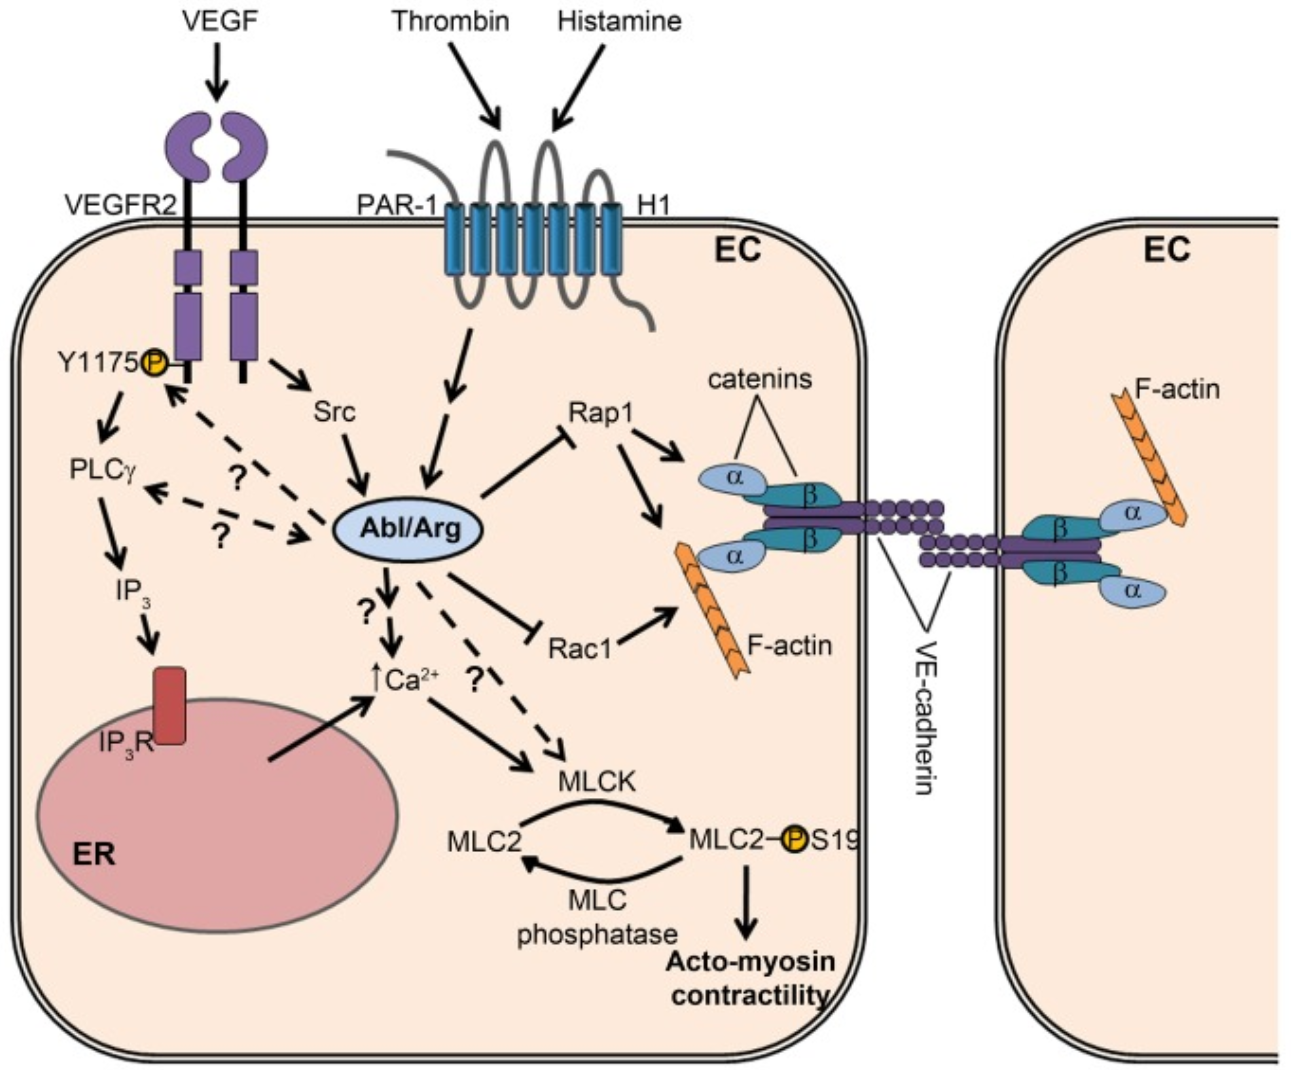
\includegraphics[width=0.5\linewidth]{figures/Inflammation/HistaminPselectin.png} 
        \caption{Overview of the histamine/thrombin cascade signaling which activates PS19 (P-selectin) to migrate up to the cell wall. This mechanism also activates the side chains VE-cadherin to open allowing for leukocytes to abandon the blood stream. Image from \href{https://www.nature.com/articles/nature13479}{"XXX UNKNOWN!"}.
        \label{figure:histamine}}
    \end{figure}  

However, histamine is also released when allergens bind to mast-cell-bound IgE antibodies sites. This is commonly known as an allergy and is the mechanism that can make your life miserable in the form of  bronchial smooth muscle contraction, urinary bladder contractions, vasodilation, visceral hypersensitivity, itch perception, urticaria, sneezing, hyper-secretion from glandular tissue, and  nasal congestion due to vascular engorgement. This is typically alleviated by the use of antihistamines medication.

In the worst-case scenario, histamine can lead to an anaphylactic shock which causes dead typically by collapsing the respiratory airways.

\subsubsection{Cytokines}

A description of the different types of cytokines can be found in section \ref{ref:inflammationCytokines}.
   
\subsubsection{Eicosanoids / Arachidonic acid}
\label{eicosanoids}

   Eicosanoids are a family of lipids that acts like hormones. They derive from arachidonic acid, and sometimes the two names are used interchangeably. Arachidonic acid is released during cell damage. Arachidonic acid is found in meat and eggs from animals that have free range and are able to exercise and move freely, as such, a lack of proper quality items in the diet can't initiate proper resolution in the inflammation cycle. They are suppressed by steroids and promoted by tissue injuries, thrombin, bradykinin, and epinephrine. An overview of the actions of eicosanoids can be seen in figure \ref{figure:Eicosanoids1}. Details regarding eicosanoids are discussed later in the sections \ref{arcachonidacidsPRO} and \ref{arcachonidacids}.
    
    \begin{figure}[ht]
        \centering
            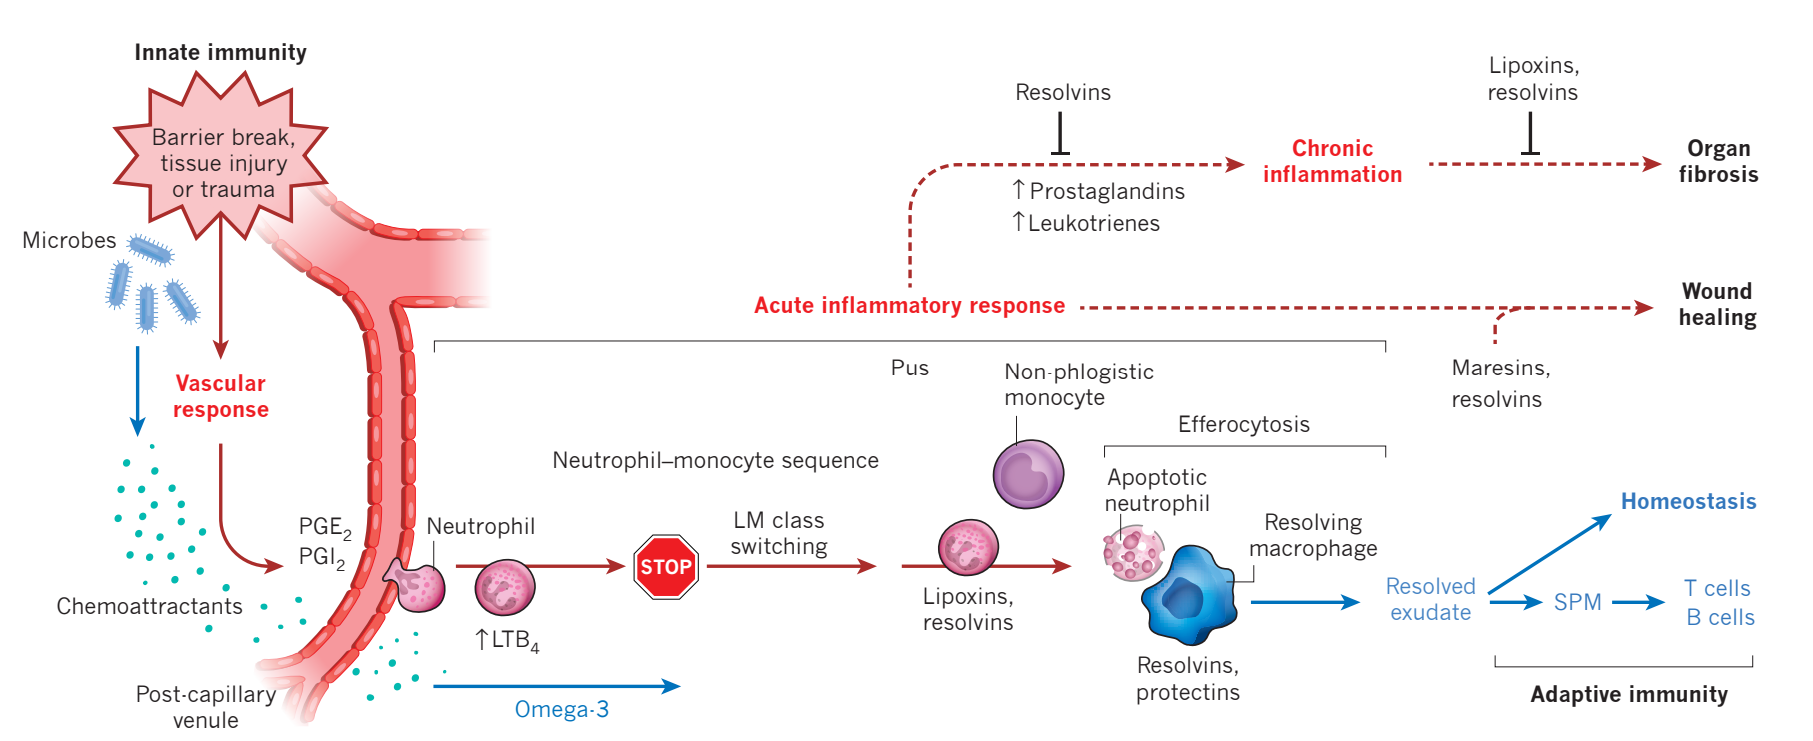
\includegraphics[width=0.9\linewidth]{figures/Inflammation/nature1.png} 
        \caption{Overview of the roles of lipid mediators in vascular and leukocyte response, from the initiation of inflammation to the resolution of the event. Image from \href{https://www.nature.com/articles/nature13479}{"Pro-resolving lipid mediators are leads for resolution physiology"}}.
        \label{figure:Eicosanoids1}
    \end{figure}  

\subsubsection{Serotonin}

Serotonin is a well-known neurotransmitter better known for regulating mood, appetite, and sleep. But it also controls the activation and proliferation of T and B cells. Overall, the function of serotonin in immunity is complex and not fully understood yet, but some studies suggest that serotonin may have a protective role against infections \cite{Roumier2019}.

\subsection{Complement system}

The complement system is a collection 32 of proteins that can kill bacteria directly, or enhance other cells in the immune system via opsonization or chemotaxis production. The functioning of the complement system is a very beautiful topic that involves the complex synchronization of proteins working together like cogs in a machine. Unfortunately is beyond the scope of this document. Here we are just going to list a simplification of the reactions present in the 3 possible pathways, highlighting the proteins important in inflammation that are mentioned in this document.

\subsubsection{Initiation}

When a couple of IgG, or a single IgM, are attached to a bacteria, is possible that by random chance a C1 protein gets attached to these antibodies. If this happens, the complement system becomes initiated.

\subsubsection{Activation}

The C1 protein has two main parts, the C1q and C1rs. C1rs is attached to the Igs, while C1q can cleave other proteins. C1q cleaves C2 making C2a and C2b, and also cleaves C4 making C4a and C4b. C4b and C2a bind together making the C4bC2a complex, which cleaves C3 making C3a and C3b. C3b binds with C4bC2a making the "C4b2a3b Convertase". This attaches to the bacteria. When this finally occurs, then it is said that the complement system is activated.

\subsubsection{Amplification}

C3b can also bind to another C3b and attach to the bacteria. This also can cleave C3 proteins, which translates into an exponential growth of the C3bC3b complex attached to the bacteria and C3a flooding the bloodstream. C3a activates basophils into releasing histamine (section \ref{in:histamine}), which promotes the expression of P-selectin, which promotes the traveling of neutrophils into the inflammation site.

\subsubsection{Termination}

C4b2a3b Convertase can also cleave C5 into C5a and C5b. C5a creates a chemotaxis gradient for neutrophils which kill the bacteria. Furthermore, neutrophils and other immune cells catch the bacteria by attaching to C3bC3b which is already attached to the bacteria wall. Here, C1q also stimulate the neutrophils to start the destruction of whatever they just grabbed. As C1q is supposed to only be attached to pathogens, this prevents them from destroying healthy cells accidentally caught by neutrophils.

The complement system can also terminate bacteria by itself forming the MAC complex, which consists of several other proteins that attach to C5b, which literally makes a hole in the bacteria wall of approximately 25 times the diameter of water molecules, allowing the insides of the bacteria to leak out.

%*****************************************
\section{Immunology advance concepts}
%*****************************************

Now that the basics of immunology have been explained, we can dive into more complex mechanism that fully explain the inflammation cycle.

\subsection{Type 1 vs Type 2 immune response}

The Type 1 immune response is characterized by the activation of Th1 cells which secrete cytokines that stimulate the production of antibodies by B cells and activation of cytotoxic T cells. It is primarily effective against intracellular pathogens such as viruses and bacteria, and the development of cell-mediated immunity. Type 1 immunity response is mainly mediated by Th1, cytotoxic T-lymphocytes, and NK cells. Type 1 immunity implies the production of pro-inflammatory cytokines and IgG and IgM antibodies.

The Type 2 immune response involves the activation of Th2 cells which secrete cytokines that activate eosinophils, basophils, and mast cells, causing allergic inflammatory responses and increased production of antibodies by B cells. It is primarily effective against extracellular pathogens such as parasites, worms, and allergens and the development of humoral immunity. Type 2 immunity response is mainly mediated by Th2 cells, eosinophils, basophils, and mast cells. Type 2 immunity generally implies the production of anti-inflammatory cytokines but also involve both types such as in the case of IL-5 which promote allergic reactions. It also mainly promotes IgA and IgE.


\subsection{Nitric Oxide}
\label{in:NO}

\ch{NO} is a free radical generated by phagocytes and is toxic to bacteria and some parasites, as well as to many human cells, leading to apoptosis. The damage to human cells is intentional and is believed to be used as a way of getting rid quickly of cells that are promoting pro-inflammation mechanisms. Is activated by \gls{ifng} and TGFα, and is suppressed by IL-4, IL-10, and TGFβ.

\subsection{JAK-STAT pathway}
\label{in:JAKSTAT}

\gls{jakstat} pathway are related to endocrinology and its main function is to couple with a receptor that attaches to the grown hormone and brings it inside the cell. However, the receptor of JAK-STAT can also bind to several cytokines. In particular IL-2, IL-6, and interferons.

What is important to understand for the scope of this document is that the JAK portion function by phosphorylating each other, which phosphorylate the STAT part, which goes into the cell nucleus, which will promote gene transcription, which promotes protein translation.

\subsection{Pro-inflammatory Eicosanoids}
\label{arcachonidacidsPRO}

In section \ref{eicosanoids} we introduced how eicosanoids are included inside granules. Here we are going to expand on them and list the pro-inflammation ones.

\subsubsection{Thromboxane}
\label{in:Thromboxane}

They work in the first stage of tissue damage by acting as a pro-coagulation agent, a vasoconstrictor, a hypertensive agent, and facilitating platelet aggregation.

\subsubsection{Prostaglandins}

\gls{pg} are a complex family of eicosanoids which act both as pro-inflammation when the recruitment of the immune system is needed, and anti-inflammatory when the damage has been resolved. There are four different subclasses:

    \begin{itemize}
        \item {\textbf{PGD2:}} Produced by mast cells and is primarily involved in allergic responses.
        \item {\textbf{PGE2:}} It is responsible for the pain and fever associated with inflammation.
        \item {\textbf{PGF2α:}} Involved in the contraction of the smooth muscle in the uterus.
        \item {\textbf{PGI2:}} Produced by the endothelial cells lining blood vessels and plays a role in vasodilation. It shares PGH2 precursors with Thromboxane which is a vasoconstrictor. You can't either have vasodilation or vasoconstriction, and both pathways are never active at the same time. Vasoconstriction reaction however occurs much more rapidly.
    \end{itemize}

\subsubsection{Leukotrienes}
\label{in:lt}

\gls{lt} are both autocrine signaling and paracrine signaling. They serve to regulate immune responses bringing neutrophils. The LTC4, LTD4, LTE4, and LTF4 prolonged slow contraction of smooth muscle and have a major bronchoconstrictor role in asthma. \gls{nsaids} block prostaglandins but promote leukotrienes, prostaglandins are initially pro-inflammatory but later on, switch to anti-inflammation, while leukotrienes are always pro-inflammation. This is the reason why NSAIDs are not always recommended for mild inflammations, and as long as the pain is bearable, is better in the long run to avoid its use. Especially if side effects on the liver and stomach are taken into consideration.

\subsection{Specialized pro-resolving mediators}
\label{arcachonidacids}
\label{in:spm}

Again, in section \ref{eicosanoids} we introduced how eicosanoids are included inside granules. Here we are going to talk about the switch from a pro-inflammation state to an anti-inflammatory effect which leads to the resolution of inflammation. These are known as specialized pro-resolving mediators (SPMs).

        \begin{figure}[h!]
            \centering
                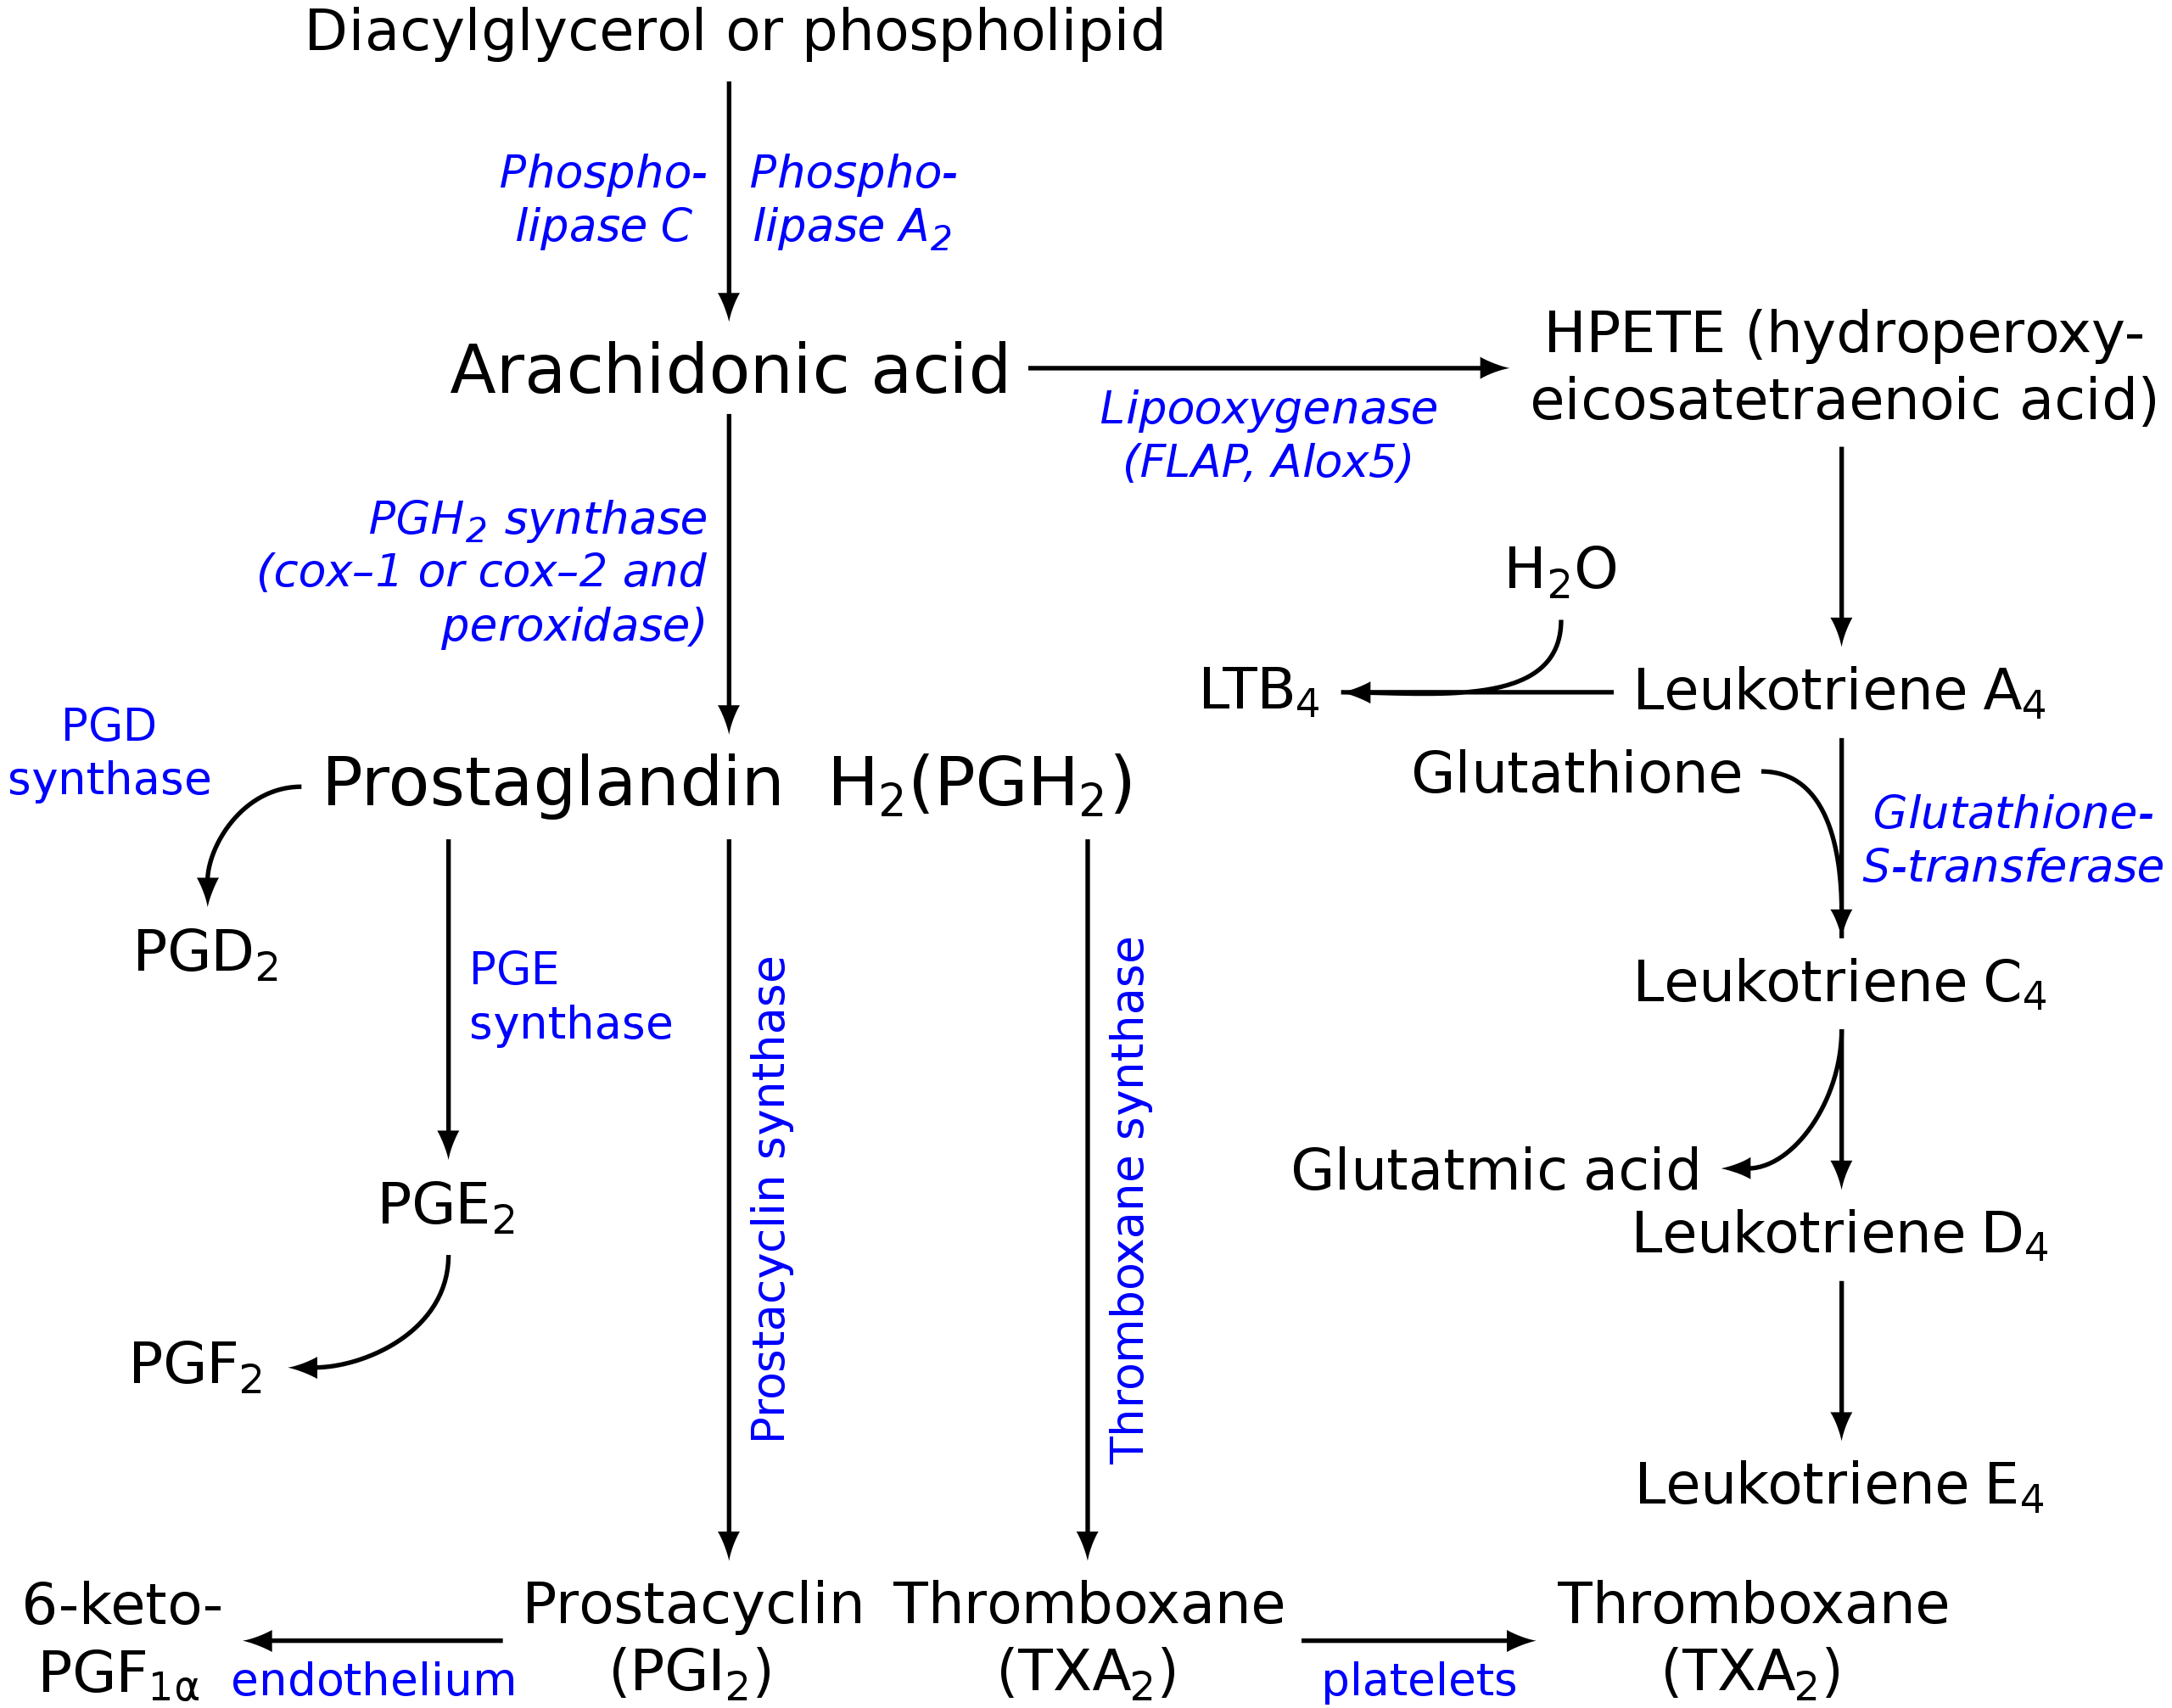
\includegraphics[width=0.7\linewidth]{figures/Inflammation/2560px-Eicosanoid_synthesis.svg.png} 
            \caption{Overview of the prostaglandin pathways. Image from \href{https://en.wikipedia.org/wiki/File:Eicosanoid_synthesis.svg}{Wikipedia}}.
            \label{figure:Phell}
        \end{figure}  


\subsubsection{Lipoxin}

Lipoxins reverse the actions of the pro-inflammatory mediators and initiate tissue repair response \cite{Basil2015}. Among many other things, they inhibit chemotaxis, transmigration, superoxide generation, NF-κB activation, generation of pro-inflammatory cytokines, suppress the production of IgM and IgG antibodies, reduce the perception of pain due to inflammation, induce the production of elements that neutralize oxidative stress and oxidant-induced tissue damage and block the actions of some leukotrienes. \cite{Sharmawalia2015}

\subsubsection{Resolvins}

Resolvins play an important role in resolving inflammation by promoting the clearance of cellular debris, bacteria, and other inflammatory mediators. They also inhibit neutrophil recruitment, decrease pro-inflammatory cytokine production, and promote tissue repair and regeneration \cite{Moro2016}. The importance of resolvins lies in their ability to control the duration and intensity of inflammation, which is crucial for preventing the development of chronic inflammatory diseases.

        \begin{figure}[h!]
            \centering
                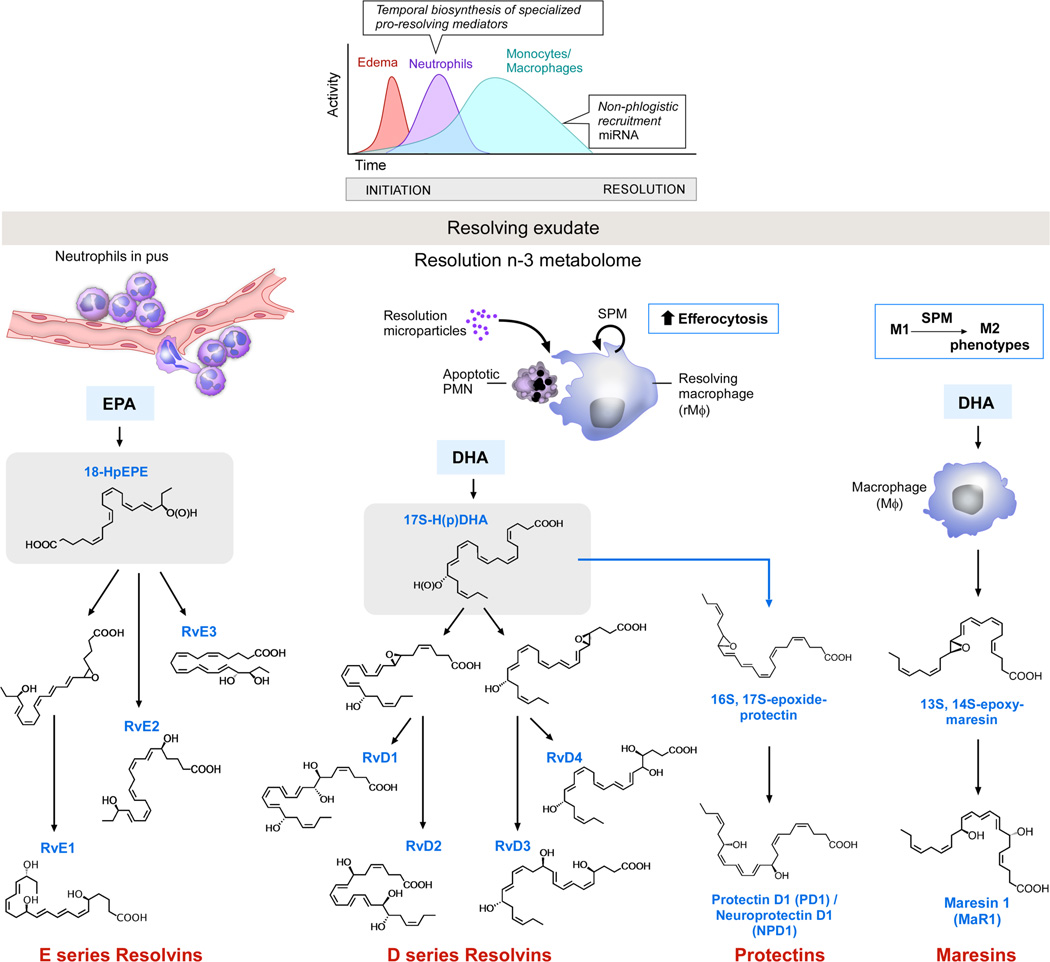
\includegraphics[width=0.8\linewidth]{figures/Inflammation/nihms646633f2.jpg}
            \caption{Overview of EPA and DHA conversion into resolvins, protectins, and maresins. Image from \href{https://www.nature.com/articles/nature13479}{"Pro-resolving lipid mediators are leads for resolution physiology"}}.
        \label{figure:Eicosanoids2}
        \end{figure}  

They are formed from the metabolism of omega-3 polyunsaturated fatty acids, in particular, \gls{epa} and \gls{dha} (figure \ref{figure:Eicosanoids2}). Humans convert \gls{ala} to EPA very inefficiently, so is recommended to take food rich in EPA directly such as salmon, mackerel, herring, cod liver, some algae, and human milk. DHA can be converted from EPA, but is recommended to also take DHA-rich food such as salmon, caviar, anchovies, mackerel, or herrings.

\subsubsection{Protectins / Neuroprotectins }

Protectins reduce inflammation induced by oxidative stress and inhibit the pro-apoptotic signal. Can potentially protect respiratory cells from viral infections. Blocks formation of pro-inflammatory prostaglandins, inhibits platelet-aggregating by thromboxane thus blocking the platelet aggregation responses such as those described for \textit{S. Aureus} in section \ref{stahp:coagulase}, and stimulate the efferocytosis \cite{Lagarde2014, Serhan2015}.

\subsubsection{Maresins}

Its name derives from \textit{\textbf{MA}crophage mediator in \textbf{RES}olving \textbf{IN}flammation}. They are involved in resolving inflammation and allergic reactions, wound healing, apoptotic human neutrophils by human macrophages, reduced lung inflammation, suppress the production of IL-5 and IL-13, and reduce the production of LTB4.

\subsubsection{Eoxins}

Eoxins are proinflammatory eicosanoids first described in 2008 \cite{Feltenmark2008} which are suggested to contribute to the inflammation of airways during allergies and some cancers \cite{Claesson2009}. They still have an unknown function in human physiology or pathology. But their production is stimulated in eosinophils by pro-inflammatory mediators PD2, LTC4, and IL-5.

\subsection{APR}

\gls{apr} are proteins that are produced by the liver and are high in plasma when there is a cause of inflammation or infection and correlate with disease activity. They are generated in response to IL-6. They go down when the cause of inflammation or infection has been resolved. However they have no diagnostic value; it is just an indicator that something wrong is going on, but there are too many diseases that cause APR to be high.

\subsubsection{CRP}

\gls{crp} is a type of APR. It is called "C" because it was first discovered reacting with the C-polysaccharide of the Capsule of \textit{Streptococcus pneumoniae}. It attaches to bacteria or dying cells which promotes phagocytosis by macrophages. It also interacts with C1q and enhances its ability to bind to pathogens, and is also believed to interact with C3; although the mechanisms of interaction between CRP and the complement system are not fully understood. It increases very rapidly and falls very rapidly as it mean half-life is barely 7 hours. Increased CRP is correlated with an increased risk of cardiovascular disease (CD) only if the patient history also correlates with CD.

\subsubsection{ESR}

The \gls{esr} is another acute phase reactant that is used to measure inflammation. It measures how quickly red blood cells clump together and settle to the bottom of a test tube. Inflammation causes the blood to become thicker and stickier, which causes the red blood cells to settle faster. In opposition to CRP, ESR still remains high after the resolution of the inflammation or infection and takes up to 7 days to regress to normal levels.


\subsection{Interleukins}
\label{in:interleukins}

% https://www.researchgate.net/figure/Role-of-interleukins-in-each-dimension-of-rheumatoid-arthritis_fig1_311472701

% https://www.researchgate.net/figure/Interleukins-involved-in-acute-and-chronic-inflammatory-responses-31-30_fig1_341541401

% https://www.researchgate.net/figure/Cytokines-profile-in-viral-infections-The-immune-response-against-viruses-initiates_fig3_330948439

% Table

% Accute VS Chronic response
% +/- immune response
% +/- inflammation
% + Cell grow
% Chemotactic
% Pyrogenic
% Released by X leukocytes
% Activate X leukocytes

% Table Agonists or Antagonists


% Figure: https://roami.ro/wp-content/uploads/2019/12/149-162_Art_Ovidiu_Farc__Victor_Cristea_web.pdf

% https://www.ncbi.nlm.nih.gov/books/NBK499840/

    \begin{figure}[h!]
        \centering
            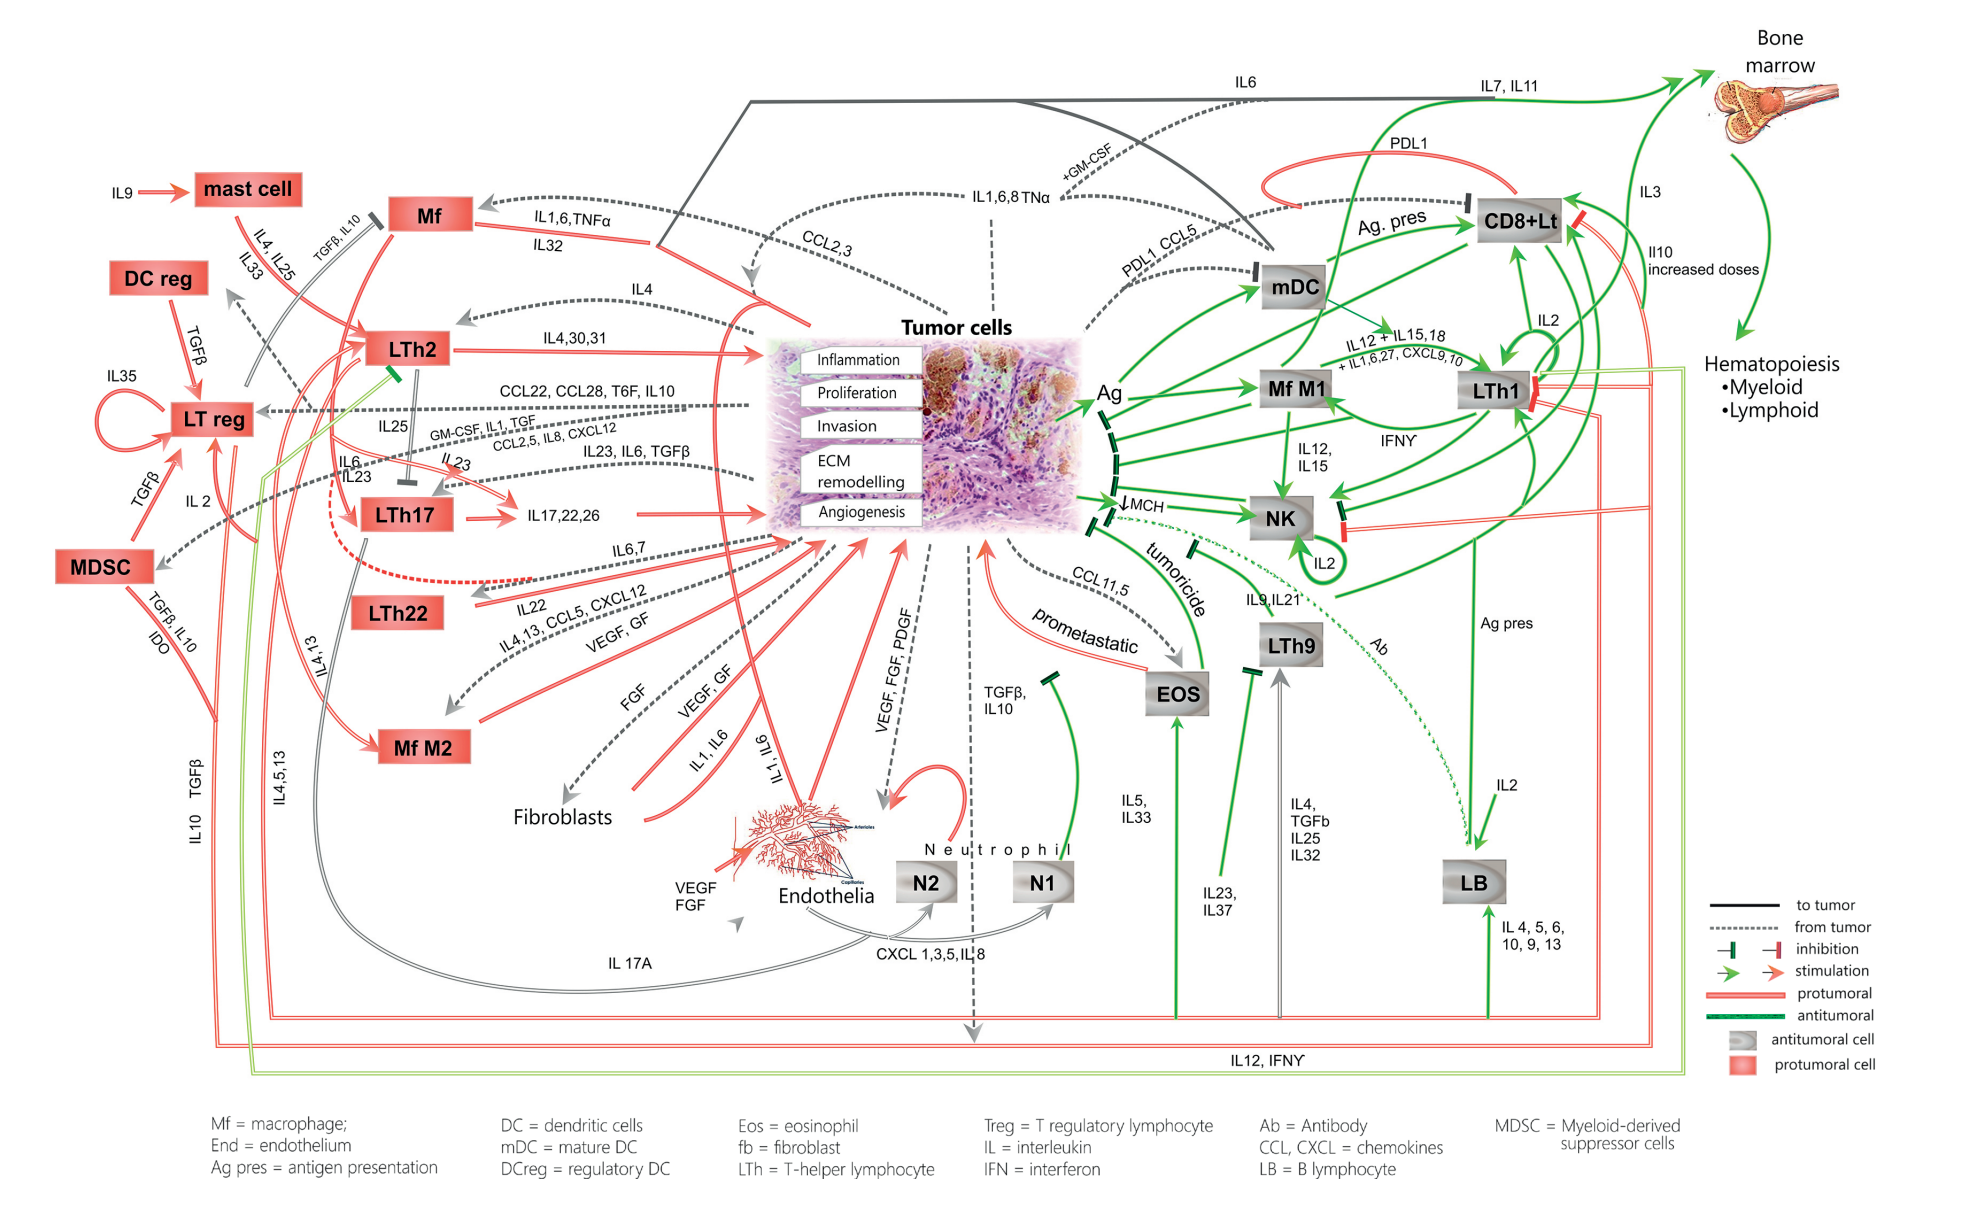
\includegraphics[width=0.8\linewidth]{figures/Inflammation/ILHell.png} 
        \caption{Overview of all interleukins affecting tumoral growth. Image reproduced from "PRO-AND ANTITUMOR ROLE OF THE INTERLEUKINS 1 TO 41" \cite{bigTumorFigureBook}}.
        \label{figure:ilhell}
    \end{figure}

Interleukin is a type of cytokine used both by the immune system and for therapeutic purposes. There are more than 50 interleukins encoded in the human genome, with several subtypes and variants. While interleukins mostly have a beneficial effect, some of them can also contribute to unwanted inflammation, autoimmune diseases, and cancer. They can stimulate or inhibit the proliferation, differentiation, activation, migration, and survival of white blood cells or other immune cells, as well as modulate the production of antibodies, chemokines, or other mediators.

The number of each interleukin is arbitrary and might lead to confusion. For example, Interleukin 1 family members includes IL-1α, IL-1β, IL-18, IL-33, IL-36α, IL-36β, IL-36γ, IL-36ra, IL-37, and IL-38. It must be taken as a unique ID with no other meaning. Here we are going to explain the function of the ILs present in the Olink panel.

The difference between interleukins can be summarized by whether they are pro or anti-inflammatory, the type of immune cells with which they interact, the type of immune cells or other human cells that produce them, and their secondary effects on the body. Individually, interleukins are very easy to understand. But their complex interactions with each other, and with other parts of the immune system make them very difficult to visualize and keep track as can be exemplified in figure \ref{figure:ilhell} and table \ref{table:ilhell}.

% Please add the following required packages to your document preamble:
% \usepackage[table,xcdraw]{xcolor}
% If you use beamer only pass "xcolor=table" option, i.e. \documentclass[xcolor=table]{beamer}

\begin{sidewaystable}[h!]% <===============================================
%\begin{table}[ht]
    \caption{Overview of all interleukins explained in this document}
    \label{table:ilhell}
    \renewcommand{\arraystretch}{1.7}
    \scalebox{0.5}{
    \centering
    \begin{tabular}{|
>{\columncolor[HTML]{FFCE93}}c c
>{\columncolor[HTML]{FBDBB5}}c ccc|}
\hline
\cellcolor[HTML]{C0C0C0}\textbf{ID}                 & \cellcolor[HTML]{C0C0C0}\textbf{Type} & \cellcolor[HTML]{C0C0C0}\textbf{Chemotactic}     & \cellcolor[HTML]{C0C0C0}\textbf{Producers}                                                                      & \cellcolor[HTML]{C0C0C0}\textbf{Targets}                                                                           & \cellcolor[HTML]{C0C0C0}\textbf{Main}      \\ \hline
\multicolumn{1}{|c|}{\cellcolor[HTML]{FFCE93}IL-1}  & \cellcolor[HTML]{FFCCC9}Pro           & \multicolumn{1}{c|}{\cellcolor[HTML]{BCFBBB}Yes} & \multicolumn{1}{c|}{Dendritic cells, Macrophages, Monocytes, T-cells}                                           & \multicolumn{1}{c|}{Pro-inflammation proteins, PGE2}                                                               & Fever, pro-apoptosis, and pro-inflammation \\
\multicolumn{1}{|c|}{\cellcolor[HTML]{FFCE93}IL-2}  & \cellcolor[HTML]{FFCCC9}Pro           & \multicolumn{1}{c|}{\cellcolor[HTML]{FBDBB5}No}  & \multicolumn{1}{c|}{NK cells, T-cells}                                                                          & \multicolumn{1}{c|}{NK cells, T-cells}                                                                             & Increases immune activity                  \\
\multicolumn{1}{|c|}{\cellcolor[HTML]{FFCE93}IL-4}  & \cellcolor[HTML]{96FFFB}Anti          & \multicolumn{1}{c|}{\cellcolor[HTML]{FBDBB5}No}  & \multicolumn{1}{c|}{Basophils, Eosinophils, Mast cells, Th2}                                                    & \multicolumn{1}{c|}{M1, Th0, Th2}                                                                                  & Make Th2 and anti-inflammation             \\
\multicolumn{1}{|c|}{\cellcolor[HTML]{FFCE93}IL-5}  & \cellcolor[HTML]{FFFFC7}Both          & \multicolumn{1}{c|}{\cellcolor[HTML]{BCFBBB}Yes} & \multicolumn{1}{c|}{Eosinophils, Mast cells, Th2}                                                               & \multicolumn{1}{c|}{Eosinophils}                                                                                   & Allergic rhinitis and asthma               \\ \hline
\multicolumn{1}{|c|}{\cellcolor[HTML]{FFCE93}IL-6}  & \cellcolor[HTML]{FFFFC7}Both          & \multicolumn{1}{c|}{\cellcolor[HTML]{BCFBBB}Yes} & \multicolumn{1}{c|}{Macrophages}                                                                                & \multicolumn{1}{c|}{B-cells, Neutrophils, T-cells}                                                                 & Fever and Autoimmune                       \\
\multicolumn{1}{|c|}{\cellcolor[HTML]{FFCE93}IL-7}  & Neither                               & \multicolumn{1}{c|}{\cellcolor[HTML]{FBDBB5}No}  & \multicolumn{1}{c|}{Stem cells / Dendritic cells /  Keratinocytes, Hepatocytes, Epithelial cells}               & \multicolumn{1}{c|}{T-cells}                                                                                       & T-cell regulator                           \\
\multicolumn{1}{|c|}{\cellcolor[HTML]{FFCE93}IL-8}  & \cellcolor[HTML]{FFCCC9}Pro           & \multicolumn{1}{c|}{\cellcolor[HTML]{BCFBBB}Yes} & \multicolumn{1}{c|}{Macrophages / Endothelial cells, Epithelial cells, Smooth muscle cells}                     & \multicolumn{1}{c|}{Neutrophils}                                                                                   & CAM activator                              \\
\multicolumn{1}{|c|}{\cellcolor[HTML]{FFCE93}IL-10} & \cellcolor[HTML]{96FFFB}Anti          & \multicolumn{1}{c|}{\cellcolor[HTML]{FBDBB5}No}  & \multicolumn{1}{c|}{Monocytes}                                                                                  & \multicolumn{1}{c|}{Macrophages, B cells, Th1}                                                                     & Anti-inflammation                          \\ \hline
\multicolumn{1}{|c|}{\cellcolor[HTML]{FFCE93}IL-12} & \cellcolor[HTML]{FFCCC9}Pro           & \multicolumn{1}{c|}{\cellcolor[HTML]{FBDBB5}No}  & \multicolumn{1}{c|}{B-cells, Dendritic cells, Macrophages, Neutrophils}                                         & \multicolumn{1}{c|}{NK cells, T-cells}                                                                             & Kill                                       \\
\multicolumn{1}{|c|}{\cellcolor[HTML]{FFCE93}IL-13} & \cellcolor[HTML]{96FFFB}Anti          & \multicolumn{1}{c|}{\cellcolor[HTML]{FBDBB5}No}  & \multicolumn{1}{c|}{Basophils, Eosinophils, Mast cells, NKT cells, Th2}                                         & \multicolumn{1}{c|}{Th0, Th2 and M1}                                                                               & Anti-inflammation and Allergies            \\
\multicolumn{1}{|c|}{\cellcolor[HTML]{FFCE93}IL-15} & \cellcolor[HTML]{FFCCC9}Pro           & \multicolumn{1}{c|}{\cellcolor[HTML]{FBDBB5}No}  & \multicolumn{1}{c|}{Dendritic cells, Macrophages, Monocytes / Fibroblasts, Keratinocytes, Myocyte, Nerve cells} & \multicolumn{1}{c|}{NK cells, Innate lymphoid cells}                                                               & Increases immune activity and survival     \\
\multicolumn{1}{|c|}{\cellcolor[HTML]{FFCE93}IL-17} & \cellcolor[HTML]{FFCCC9}Pro           & \multicolumn{1}{c|}{\cellcolor[HTML]{FBDBB5}No}  & \multicolumn{1}{c|}{Th17}                                                                                       & \multicolumn{1}{c|}{B-cells, Monocytes, Neutrophils, T-cells /  Epithelial cells, Endothelial cells,  Fibroblasts} & Increases pro-inflammatory cytokines       \\ \hline
\multicolumn{1}{|c|}{\cellcolor[HTML]{FFCE93}IL-18} & \cellcolor[HTML]{FFCCC9}Pro           & \multicolumn{1}{c|}{\cellcolor[HTML]{FBDBB5}No}  & \multicolumn{1}{c|}{Several}                                                                                    & \multicolumn{1}{c|}{Several}                                                                                       & Type 1 immunity                            \\
\multicolumn{1}{|c|}{\cellcolor[HTML]{FFCE93}IL-20} & \cellcolor[HTML]{FFCCC9}Pro           & \multicolumn{1}{c|}{\cellcolor[HTML]{BCFBBB}Yes} & \multicolumn{1}{c|}{Dendritic cells, Granulocytes, Monocytes}                                                   & \multicolumn{1}{c|}{Adipocytes, Endothelial cells, Keratinocytes}                                                  & Healing                                    \\
\multicolumn{1}{|c|}{\cellcolor[HTML]{FFCE93}IL-22} & Neither                               & \multicolumn{1}{c|}{\cellcolor[HTML]{FBDBB5}No}  & \multicolumn{1}{c|}{Macrophages, Neutrophils, NKT cells, Th1, Th17}                                             & \multicolumn{1}{c|}{Several}                                                                                       & Healing and germicidal                     \\
\multicolumn{1}{|c|}{\cellcolor[HTML]{FFCE93}IL-24} & \cellcolor[HTML]{FFCCC9}Pro           & \multicolumn{1}{c|}{\cellcolor[HTML]{FBDBB5}No}  & \multicolumn{1}{c|}{Macrophages, Monocytes, Th2}                                                                & \multicolumn{1}{c|}{Several}                                                                                       & Anti-healing and Anti-cancer               \\ \hline
\multicolumn{1}{|c|}{\cellcolor[HTML]{FFCE93}IL-33} & \cellcolor[HTML]{96FFFB}Anti          & \multicolumn{1}{c|}{\cellcolor[HTML]{FBDBB5}No}  & \multicolumn{1}{c|}{Several}                                                                                    & \multicolumn{1}{c|}{Mast cells, Th2}                                                                               & Promotes Th2 cytokines                     \\ \hline
\end{tabular}
    }
%\end{table}
\end{sidewaystable}

\subsubsection{IL-1}
\label{in:IL1}

\gls{il1} is a cytokine that is involved in regulating the immune response and inflammation. It is produced by macrophages, monocytes, dendritic cells, and certain types of T cells. It is involved in both innate and adaptive immune responses and plays a key role in the body's defense against pathogens.

Activates and promote the production of several proteins involved in the acute phase of inflammation. In particular highlights that activates PGE2 which leads to fever, and it increases the concentration of TNF and IL-1 in the brain which may break the blood-brain barrier. Increases APR. It also triggers the production of chemokines, activates T-cells, and promotes B-cells maturation and proliferation. It also promotes IL-2 and fibroblast growth factors.

There are two main forms of IL-1: IL-1 alpha and IL-1 beta. While they are both involved in the same functions, they are produced by different cells and are regulated differently:

\begin{itemize}

    \item {\textbf{IL-1}} alpha is produced and stored by epithelial cells, endothelial cells, and fibroblasts. IL-1 alpha is stored in the cytoplasm of cells, which means that it can be released rapidly in response to stress or injury.
    
    \item {\textbf{IL-1}} beta is produced when needed and is not stored. Is secreted by activated monocytes and macrophages. IL-1 beta is produced as an inactive precursor.

\end{itemize}

Both of them need to be activated, which is a role primarily done by the caspase family of proteins. Caspase-8 is one of the proteins which we use in our analysis and is explained in section \ref{in:olink-casp8}.

Steroids can block IL-1, which is of special interest in the treatment of autoimmune diseases.

\subsubsection{IL-2}
\label{in:IL2}

\gls{il2} is produced mainly by activated T cells and NK cells. IL-2 functions as a growth factor for Th, cytotoxic T cells, and regulatory T cells, promoting their proliferation and activation. It also activates NK cells and cytotoxic T cells, increasing their cytotoxicity (ability to kill infected or cancerous cells).

The \gls{il2r} is the receptor complex that binds and responds to IL-2. It is expressed on the surface of T cells, NK cells, B cells, and dendritic cells. IL-2R mediates signaling through various intracellular pathways, including the JAK-STAT pathway. The signaling regulates gene expression, cell proliferation, survival, and differentiation in response to IL-2. IL-2 can also bind to the IL-12 receptors which will be discussed later, but in essence further promotes Th1 and NK cells.

Changes in IL-2R expression and signaling can impact immune cell function and contribute to immune dysfunction and disease.

%\subsubsection{nnIL-3}
%\label{in:IL3}

%Bone marrow stem cell differentiation

\subsubsection{IL-4}
\label{in:IL4}

This induces differentiation from Th0 to Th2 and the production of IL-4 Th2 cells, which creates a positive feedback loop. IL-4 is also produced by mast cells, eosinophils, and basophils.

Secondary functions include decreasing the production of Th1 because Th0s are converted to Th2s instead. M1 macrophages are also decreased and promoted into M2 instead. IL-4 is usually coupled with secretion of IL-10 and TGF-β which further reduce inflammation and M2 production. It also decreases the production of IFNγ. By decreasing Th1 indirectly decreases IL-12 also.

Its functions are similar to those of IL-13. Overproduction of IL-4 is related to allergies.

\subsubsection{IL-5}
\label{in:IL5}

It is primarily produced by Th2 cells, mast cells, and eosinophils. It activates, stimulates, differentiates, and recruits eosinophils. It also makes B cells focus producing IgA. It has been associated with allergies, in particular with allergic rhinitis and asthma.

It can also suppress the production of pro-inflammatory cytokines, TNF-α and IL-1β, reducing the activation of inflammatory cells.

\subsubsection{IL-6}
\label{in:IL6}

Is a cytokine that plays a variety of roles in the body. It acts as a pro-inflammatory cytokine and as an anti-inflammatory myokine; this is a type of signaling that occurs in the skeletal muscle cells which has an effect on nearby cells as well as the endocrine system. In particular, it inhibits the effects of TNF-α and IL-1.

Is produced by macrophages in response to \gls{pamps}. IL-6 initiates PGE2 production which leads to fever. Furthermore, in muscle and fatty tissue increase energy consumption leading to increased body temperature. It also has an influence on the liver increasing APR, and is believed to be the reason why obese individuals have higher CRP. This is closely related to long-term inflammation due to obesity.

IL-6 is responsible for stimulating acute phase protein synthesis, as well as the production of neutrophils in the bone marrow. It supports the growth of B cells and is antagonistic to regulatory T cells.

IL-6 stimulates the inflammatory response in multiple auto-immune processes, such as MS, \gls{nmosd}, diabetes, lupus, atherosclerosis, rheumatoid arthritis, and many more.

As a myokine, it suppresses inflammation caused by stress in bones and muscles during exercise and promotes bone re-absorption. Myokines function is still poorly understood but is believed to have a beneficial impact as a response to PA \cite{Ostrowski2000} which is related to IL-10 too. Furthermore, IL-6 also regulates glucose metabolism and energy homeostasis.

\subsubsection{IL-7}
\label{in:IL7}

It is secreted by stem cells, keratinocytes, dendritic cell, hepatocyte and epithelial cells. It stimulates the differentiation of stem cells into the lymphoid path (NK cells, B cells, and T cells) as oppose to IL-3 which stimulate the opposite branch. However elevated levels of IL-7 promotes acute lymphoblastic leukemia and T cell lymphoma. Furthermore, it plays a critical roll in the survival of T cells and their development in the thymus.

\subsubsection{IL-8 / CXCL8}
\label{in:IL8}

It is also known as neutrophil chemotactic factor. It name has officially changed to CXCL8. IL-8 main mission is to attract neutophils into infection sites, but it also works upon other granulocytes. Is produced by any cells with toll-like receptors that are involved in the innate immune response; but mainly macrophages, epithelial cells, muscle cells in the airway passage, and endothelial cells.

IL-8 is readily stored in Weibel-Palade bodies of endothelial cells and has an quick response time. It increases intracellular calcium ions, histamine release, and ROS, and the expression of CAMs (section \ref{in:selectin}).


\subsubsection{IL-10}
\label{in:IL10}

IL-10 and its receptor play a very influential role in the anti-inflammation process and overall it should considered as such. However it can also promote pro-inflammatory effects stimulating B cells activity. It activity is related also to IL-19, IL-20 and IL-24.

It produced primarily by monocytes, but also secondarily by Th2, mast cells, regulatory T cells, and activated T cells and B cells.

It has 4 receptors in total which can down-regulate the JAK-STAT activation and block NF-κB activity. They are present in Th1, macrophages, B cells, and their function is predominantly stop pro-inflammation activity. In Th and some macrophages cells it down-regulate the production of pro-inflammatory cytokines TNFα, IL-1β, IL-2, IL-3, IL-12 and other not discussed in this document. In cells with TLRs can block the production of IFNγ. On CD4+ cells can suppress their antigen expression which was discussed in section \ref{inf:cd4cdprotein}. On bacteria can directly inhibits \gls{lps}.

Another important aspect of IL-10 is that promotes the COX activation shown in figure \ref{figure:Phell}, suppressing LT production and enhancing PG which in time promotes the SPMs discussed in section \ref{in:spm}.

Finally, also comment that PA increases the levels of IL-10 by about 30x \cite{Ostrowski1999} and seems to be linked with IL-6, suggesting that PA promotes an anti-inflammation environment in the body.

\subsubsection{IL-12}
\label{in:IL12}

IL-12 is produced by dendritic cells, macrophages, neutrophils, and B-cells. It receptors can be found on T cells and NK cells.

It main function is to promote as much killing as possible. It increases Th1 activity which increases macrophages and cytotoxic T cells. It also increases NK activity. IL-2 can also bind to the IL-12 receptors adding to this effect. It also stimulates the production of IFN-γ, TNF-α, and override the activity of IL-4.

\subsubsection{IL-13}
\label{in:IL13}

Produced by Th2, CD4, natural killer T cells, mast cells, basophils, and eosinophils.

Is an interleukin very similar to IL-4. IL-13 can bind to both IL-4 receptors and IL-13 receptors. However IL-13 lack the same ability to differentiate Th0 to Th2. Instead it specialize more in the airway hyperresponsiveness and mucus production proper of allergies.

\subsubsection{IL-15}
\label{in:IL15}

Produced by monocytes, macrophages, dendritic cells keratinocytes (skin), fibroblasts (extracellular matrix), myocyte (muscles) and nerve cells.

Is an interleukin very similar to IL-2. But unlike the IL-4 / IL-13 pair, in this case IL-15 can only bind with it own receptor which is expressed in a wider range of cells; lymphocytes and NK cells. IL-2 activates cells, while IL-15 promotes the survival and activation of the same cells, plus those extra with IL-15 receptor.

\subsubsection{IL-17}
\label{in:IL17}

It is produced by many type of both immune and non-immune cells, but primarily by Th17 cells in order to initiate the adaptive immune response against bacteria or fungi.

The IL-17 receptors expression has been found on T cells, B cells, monocytes, neutrophils, epithelial cells, fibroblasts, and endothelial cells. Interleukin 17 has 5 known types of receptors (IL17RA, IL17RB, IL17RC, IL17RD and IL17RE). The main difference between them is which type of cell express each. IL-17RA is the most widely expressed and can also bind with other IL of the IL17 family. The mechanisms of each of the receptor is very complex which include the activation of pathways not even mentioned in this document, and as such, they are not going not be described further. However it will be mention that they are the target of several drugs for IL-17 inhibitor and monoclonal antibodies techniques which aim for the treatment of several autoimmune diseases.

\subsubsection{IL-18}
\label{in:IL18}
% I really don't understand what IL-18 is doing or why the receptors are important -_-

Is produced by many types of cells in the body, and it receptor is also found in big variety of cells. IL-18 is involved in the activation of NK cells, T cells, and B cells. The binding of IL-18 to IL-18 receptor activates NF-κB which promotes the production of pro-inflammatory cytokines in both immune and non-immune cells.


\subsubsection{IL-20}
\label{in:IL20}

IL-20 is mainly produced by monocytes, granulocytes, and dendritic cells in response to IL-1β, IL-17, IL-22, TNF, and LPS. The main targets of IL-20 are keratinocytes, endothelial cells, and adipocytes. It plays a role in several biological processes:

\begin{itemize}

    \item Regulation of skin homeostasis: IL-20 is produced by skin cells and helps to regulate the normal function of keratinocytes and fibroblasts. It can also modulate the expression of various genes involved in skin development and differentiation.
    
    \item Wound healing and tissue repair: IL-20 has been shown to stimulate the proliferation and migration of epithelial cells, which play a critical role in wound healing and tissue repair. It can also enhance the production of collagen and other extracellular matrix proteins, which are essential for tissue regeneration.
    
    \item Cancer development: Because it promotes tissue grow, specially in the skin, it can also promote development of tumor cells which derives from the skin. However it also known to reduce tissue damage in chronic inflammation which suppress cancer. So the mechanism of IL-20 with respect cancer is ambiguous and needs further study.
    
    \item Inflammatory responses: IL-20 can stimulate the production of TNFα, IL-1I, L-6 and IL-8, leading to an pro-inflammatory response. It also a chemotaxin itself. Can modulate the function of dendritic cells, T cells, and B cells. It can also regulate the production of antibodies
    
\end{itemize}






%\subsubsection{nnIL21}
%\label{in:IL21}

%Chemotaxis, attract neutrophils

\subsubsection{IL-22}
\label{in:IL22}

IL-22 is produced by the immune cells Th1, Th17, NKT cells, neutrophils and macrophages, which are already in the inflammation site. It targets several non-immune cell types. It promotes cell grown and healing of tissue, while at the same times promote the synthesis of several proteins with germicidal properties.

%Chemotaxis, attract neutrophils

\subsubsection{IL-24}
\label{in:IL24}

Released mainly by activated monocytes, macrophages and Th2 cells through TLR. Target cells are those in skin, lung, and reproductive tissues. It suppress cell proliferation during wound healing, and particularly is has been found to have an important role in destroying cancerous cells. It promotes TNF-α, IFNγ, and IL-1, which in term promote cell's apoptosis.

\subsubsection{IL-33}
\label{in:IL33}

It is expressed by a wide variety of cells. It can target IL1 family receptors mainly expressed in Th2 cells and mast cells.

IL-33 main function is to promote Th2 cytokines production. This has anti-inflammatory effects such as those described in IL-4, but also pro-inflammatory effects due allergic reactions as described for IL-13. But overall, same as with IL-4 and IL-13, is an anti-inflammatory cytokine that leads to resolution. IL-33 is known to play an important role in the development of allergies and asthma. It activates Th2 cells and eosinophils, which are the key mediators of allergic inflammation. IL-33 also contributes to airway remodeling, mucus production, and bronchoconstriction.

IL-33 has both pro-tumor and anti-tumor effects depending on the type and stage of cancer. In some cancers, IL-33 promotes tumor growth and metastasis by stimulating angiogenesis and cell proliferation. However, in other cancers, IL-33 promotes anti-tumor immunity by activating natural killer cells and CD8+ T cells.

\subsection{Interferon}
\label{in:inter}

Interferon is the way cells have to communicate to other cells that a virus is about to kill them, and they need to be ready and prepared so they don't die next. If a virus manages to sneak its RNA/DNA into a cell, it usually means that the cell is unsalvageable and needs to be eliminated. The cell itself can recognize this. The cell will initiate the \gls{irf} by two means. First it can recognize viral parts using its own \gls{prrs}. The second way is using cGAS–STING cytosolic DNA sensing pathway; this tool detect DNA in the cytosol of the cell. DNA should never be outside the nucleus, so chances are that DNA in the cytosol is viral DNA and needs to be eliminated. Either way, this activation leads to further activation of NF-κB in activated B cells.

\subsubsection{Alpha and Beta interferons}

IRF will stimulate the cell DNA to express \gls{ifna} and \gls{ifnb} which will be released from the cell and go into nearby similar friendly cells and NK cells.

On similar cells IFN-$\alpha$ and IFN-$\beta$ will stimulate the differentiation of protein kinase R. This protein clip viral RNA/DNA, so when the virus that was lurking around injects its genetic material into the cell, protein kinase R will be ready to cut it and make it useless. On the other hand, it also alerts nearby NK cells to come by and start checking the MHC1s. The infected cell will usually fail to provide a valid MHC1 and the NK cell will eliminate it.

Finally, IFN-$\alpha$ and IFN-$\beta$ also leads to the activation of the JAK-STAT pathway (section \ref{in:JAKSTAT}), which leads to the activation of downstream \gls{isgs}, which leads to the production of more interferons creating a local positive-feedback loop which alert many nearby cells at once.

\subsubsection{Gamma interferon}
\label{in:ITFG}

IRF will also stimulate the expression of \gls{ifng}. IFNγ is produced mostly by NK, NKT, CD4 Th1, and CD8 cytotoxic T lymphocytes. Its function is to activate nearby macrophages, signaling them to start proliferating and to express even more MHC1/2 on the surface so they can communicate with other leukocytes better. Macrophages can also release IFN-$\alpha$ and IFN-$\beta$. It can also activate dendritic cells and B-cells, and induce production of TNF-α and IL-6.

An important property of IFNγ is that can increases the production of CXCL10 which is an anti-angiogenic chemokine that will be discussed later. In essence it means that IFNγ aids in suppressing the creation of new blood vessels. This suppress healing, but also suppress tumor grow and is an important 

\subsection{Toll like receptors}

\gls{tlrs} are a group of membrane receptors that are expressed on APC that enhance inflammatory response. They bind to PAMPs, and depending on which type of TLR was binding to which type of PAMP, they will signal the production of certain cytokines or chemokines. There are 13 known TLRs, 10 of which are present in humans.

    \begin{figure}[ht]
        \centering
            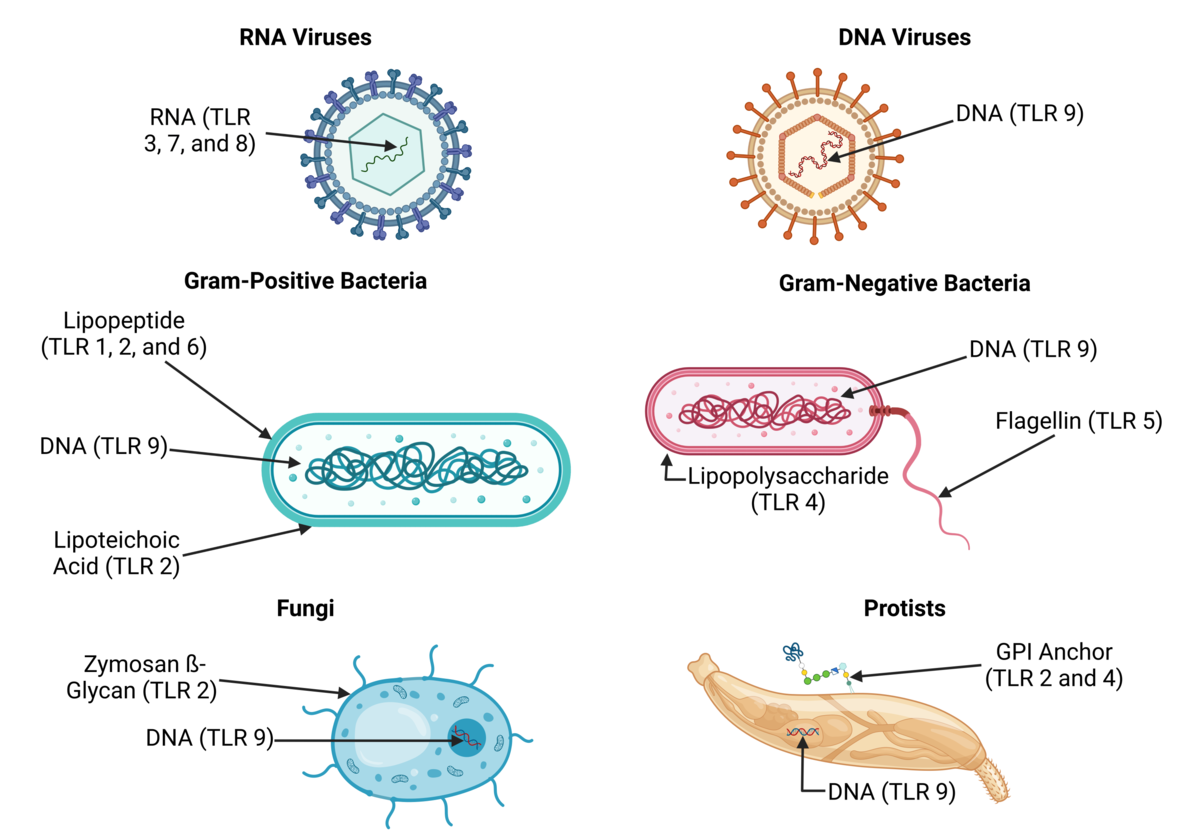
\includegraphics[width=0.7\linewidth]{figures/Inflammation/Toll-Like_Receptors_(TLRs).png } 
        \caption{Overview of factors that activate human TLR. Reproduced from \url{https://wikimedia.org}}
        \label{figure:TLRhell}
    \end{figure}

There are three main gene regions that are activated by TLRs:

\begin{itemize}
    \item \gls{ap1} which regulates transcriptions of several cytokines and growth factors. Furthermore, it controls many cell processes including differentiation, proliferation, and apoptosis.    
    \item IRF (discussed in section \ref{in:inter}) 
    \item NF-κB (discussed in section \ref{inf:nfkb})
\end{itemize}

TLR activation can also lead to excessive inflammation and tissue damage, thus dysregulation of TLR signaling has been implicated in various inflammatory disorders and autoimmune diseases.

\subsection{Tumor necrosis factors superfamily}
\label{in:tnf}

The tumor necrosis factor (TNF) superfamily is a collection of 19 proteins. These proteins are mostly expressed in immune cells and they regulate immune response, inflammation, proliferation, differentiation, apoptosis, and embryogenesis. Besides all of that, they can also leave the cell and act as cytokines. Here we are going to discuss the 3 major ones that interact with many other parts of the immune system, while in the Olink panel section, we will see the details of other TNFs and TNF receptors.


\subsubsection{LTα / TNFβ / TNFSF1}
\label{inf:tnfb}

\gls{lta} mainly acts as a lymphoid tissue organizer by promoting the development and maintenance of secondary lymphoid organs such as lymph nodes and spleen. LTα can also signal through the \gls{ltbr} to stimulate the production of pro-inflammatory cytokines and chemokines by stromal or epithelial cells.

This protein was formally known as Tumor Necrosis Factor β, and is referred to as such in the Olink panel.

\subsubsection{LTβ / TNFC / TNFSF3}

\gls{ltb} is involved in the regulation of immune cell trafficking and inflammatory responses. LTβ can bind to three distinct receptors: LTβR, TNF receptor 2 (TNFR2), and \gls{hvem} (also known as TNFRSF14). The binding of LTβ to LTβR promotes the development of lymphoid tissues and contributes to the initiation of adaptive immune responses. The binding of LTβ to TNFR2 or HVEM can activate NF-κB signaling and induce the expression of pro-inflammatory genes.

This protein was formally known as Tumor Necrosis Factor C.

\subsubsection{TNF / TNFα / TNFSF2}
\label{inf:tnfa}

The name for this protein might be confusing. Tumor Necrosis Factor is protein 2 of the many Tumor Necrosis Factor superfamily proteins (TNFSF2). Now it is called simply Tumor Necrosis Factor. It was formerly known as tumor necrosis factor-alpha (TNFα) and is referred as such in the Olink panel and throughout this thesis to avoid misunderstandings with the TNF superfamily.

It shares many biological functions and signaling pathways with LTα and LTβ. TNFα is produced by a variety of immune and non-immune cells in response to infections, tissue damage, or other inflammatory stimuli, but in particular, it is chemotaxis that attracts neutrophils and promotes leukocytosis. It will increase APR, and it causes fever by activating PGE2.

TNFα can bind to two receptors: TNFR1 and TNFR2, which are expressed in almost all cell types. The binding of TNFα to its receptors triggers a cascade of signaling events that lead to the activation of inflammatory pathways, cell proliferation, and cell death.

It also acts as an adipokine. TNFα promotes insulin resistance. This is a condition in which higher levels of insulin are present in the bloodstream, but they are unable to move efficiently glucose into the cells for energy. As such is associated with obesity-induced type 2 diabetes.


%*****************************************
\section{Inflammation cycle}
\label{in:cycle}
%*****************************************

We have finally reached the point in which we can understand everything that happens during an inflammation event. An inflammation will start with a specific stimulus, and from there on all the mechanisms that lead to inflammation and the resolution of inflammation will take place at the same time. However some will act faster than others; first, the clotting of the blood happens very quickly, then the inflammation and destruction of the pathogen happen, and finally, the mechanisms for resolution will mount up and decrease the inflammation.

\subsection{Stimuli}

In order to start an acute inflammation process is necessary to provide the body with a stimulus, for example, pathogens, toxins, radiation, or physical trauma. The stimuli can be classified as:

\begin{itemize}

    \item {External:}

        \begin{itemize}
    
            \item{Non-microbial}

                \begin{itemize}
            
                    \item {Allergens} are a type of antigens that stimulate the secretion of IgE to fight a particular allergen instead of a normal parasitic infection. This includes plants, metals, insect stings, penicillin, many types of food, vaccines, animals, and many more.
                    
                    \item {Irritants} can be any object that enters the body and causes irritation, such as splinters and dirt. It can also be substances such as acids, alkalis, and solvents.
                    
                    \item {Toxic compounds} like chemicals such as recreational drugs or snake venoms, physical, such as coal dust or asbestos, or ionizing radiation.
    
                \end{itemize}
            
            \item{Microbial}

                \begin{itemize}
            
                    \item{Virulence factors}, such as everything discussed in chapter \ref{ch:staph} regarding \textit{S. Aureus} colonization, immunoevasion, and immunosuppression.
                    
                    \item{\gls{pamps}}. These are small molecule patterns present in pathogens but not the host, which help the immune system target the pathogens. Common PAMPs are found in:

                        \begin{itemize}
                    
                            \item Viruses: double-stranded RNA (dsRNA)
                            
                            \item Gram-Negative bacteria: \gls{lps} and Peptidoglycans described in section \ref{staph:OuterMembrane}.
                            
                            \item Gram-Positive bacteria: Lipoteichoic acid and bacterial lipoproteins (sBLP) described in section \ref{staph:gram-types}.

                        \end{itemize}

                \end{itemize}

        \end{itemize}

    \item {Internal:}. \gls{damps} are host cell molecules that are released when there is tissue damage, or the cell just dies.
            
\end{itemize}

These factors are not mutually exclusive. For example, a bacteria can have PAMPs, and start destroying human cells which then will release DAMPs. Irritants don't contain PAMPs, but in contact with the skin, they can form a complete antigen and cause inflammation, like with for example poison ivy.

\subsection{Clotting}

When an injury occurs, even before dealing with any infection, is necessary to stop the bleeding so you don't die from blood loss. The first step in blood clotting is the formation of a platelet plug, which aggregates at the site of injury and becomes activated, causing them to stick together and form a temporary seal over the site of the injury. As platelets aggregate, they release \gls{vwf} (section \ref{in:VonWill}) so they can stick together, and thromboxane (section \ref{in:Thromboxane}) to reduce blood flow to the site of injury. This form a quick temporal fix that prevents further bacteria from entering the body and provides the basic structure for tissue repair.

Once the platelet plug has formed, a more stable blood clot is formed later on using proteins called clotting factors. These clotting factors work together to convert prothrombin, into thrombin, which in turn converts fibrinogen into fibrin. Fibrin forms a net that reinforces the platelet plug, creating the final stable clot. Fibrin also happens to help \textit{S. Aureus} infiltration as described in section \ref{staph:Fibrin}.

\subsection{Acute phase}

Once the clot is in place, then its possible to activate vasodilation and bring in the immune system so it can deal with the infection. Leucocytes have external \gls{prrs} in the cell surface which are activated in contact with PAMPs or DAMPs, which trigger the immune and inflammation response. These PRRs are non-specific, meaning that the leucocyte doesn't know what causes the stimuli, just that something bad is happening and an immune response needs to happen to whatever it is. There is also no cell memory associated with the PRRs.

Additionally, some non-immune cells such as epithelial cells, endothelial cells, and some stromal cells can also express certain types of PRRs that can recognize viral components such as \gls{tlrs} or \gls{rlrs} which are explained in section \ref{in:inter}.

    \begin{figure}[h!]
        \centering
            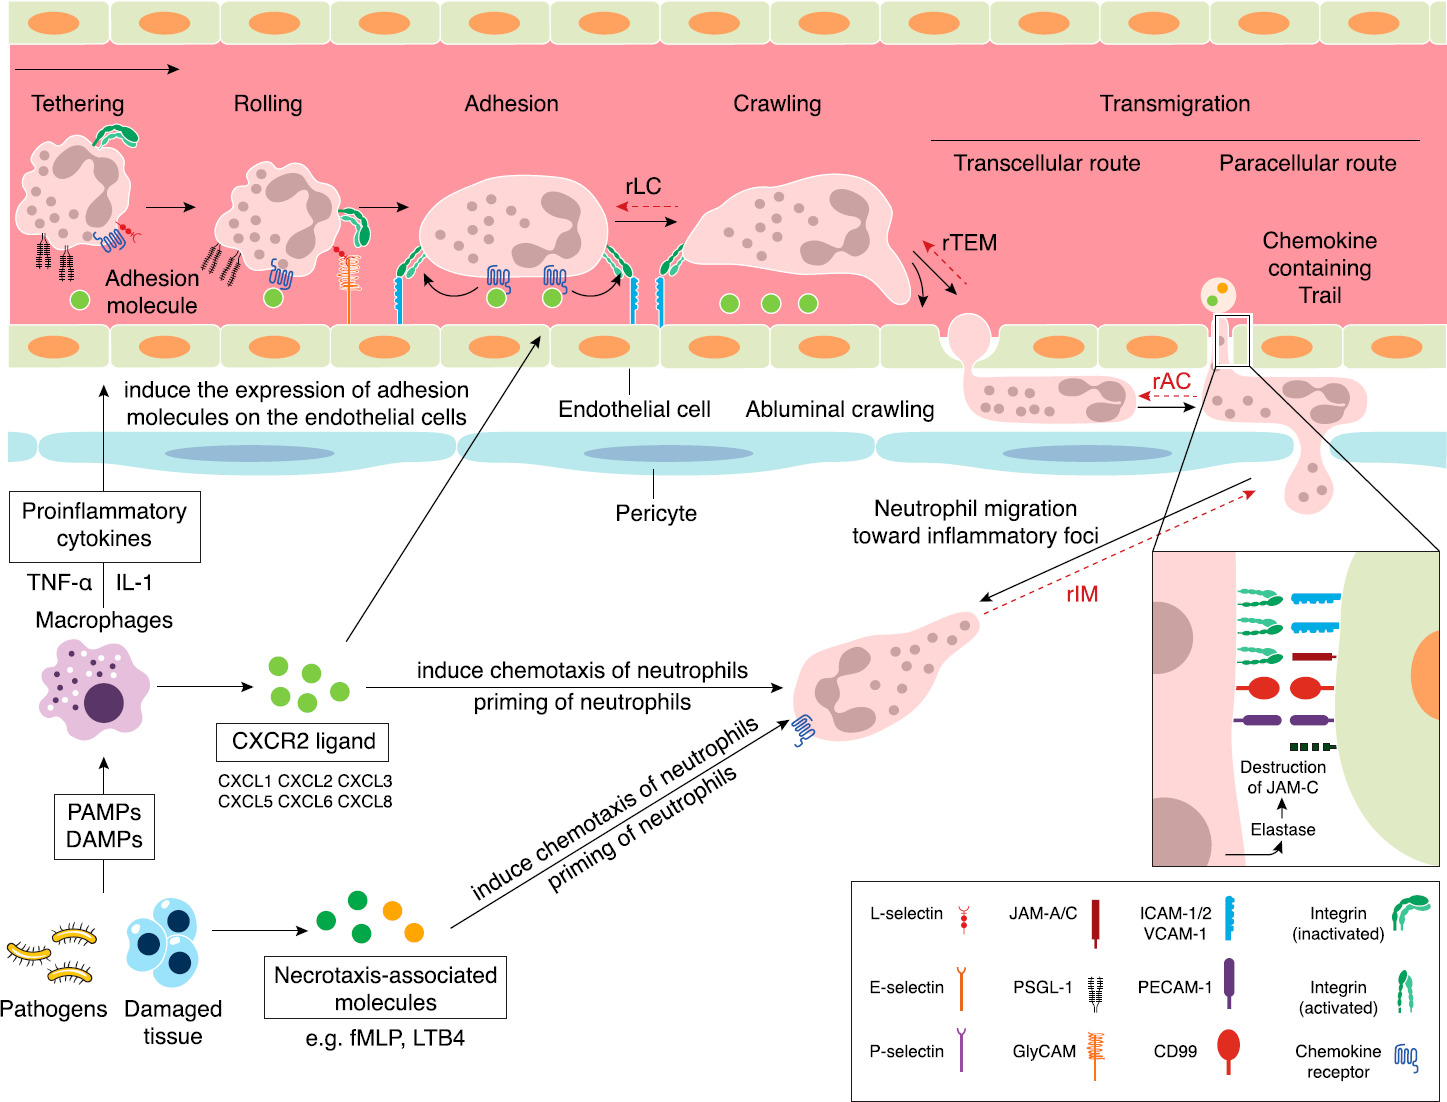
\includegraphics[width=0.8\linewidth]{figures/Inflammation/jlb0617-fig-0002-m.jpg} 
        \caption{Overview of a cell migration from a blood vessel to an inflammation site. Image reproduced from "Deep insight into neutrophil trafficking in various organs" \cite{Hyun2017}}.
        \label{figure:inflammationStarts}
    \end{figure}  

When PAMPs interact with a granulocyte as described in section \ref{inf:granules} , they release histamines, bradykins, and eicosanoids that cause vasodilation in blood vessels and also open a gap in the endothelium releasing blood into the area close to where the DAMP activity is happening, which causes swelling. It also causes muscle relaxation which causes vasodilation (localized hyperemia). You get more blood in the area which turns the area red. It also helps endothelium cells to express more selectins which attract neutrophils to the inflammation site via extravasation. Then neutrophils phagocytose the bacteria. Then dendritic cells present pieces of the bacteria to T-Lymphocytes which activates the adaptative immune system if necessary. 

\subsection{Switching and resolution}

Specialized pro-resolving mediators (SPM) are produced to inhibit pro-inflammatory mediators and regulate neutrophils. This mechanism is done by the Lipid-mediator-class switching illustrated in figure \ref{figure:Eicosanoids1} which is described in sections \ref{arcachonidacidsPRO} and \ref{arcachonidacids}.

\subsection{Tissue repair}

Macrophages eat dying or dead cells which provide room for new cells. They also secrete growth factors that promote the angiogenesis of temporal capillary vessels. Fibroblasts synthesize collagen in the area of interest. Mild damage in a tissue gets repaired to a normal state, while in severe damage the tissue is replaced by a non-functional fibrous scar.

\subsection{Chronic inflammation}

If everything goes well, the infection has been neutralized, and the inflammation has subsided. However, sometimes errors can occur. Typically this involved not being able to clear the site of inflammation from the cause. For example DAMPs or any other bacterial debris. In worse cases, external bodies such as undetected wood splints, or metal allocated inside the muscle that can't be removed surgically.

Dysregulation of cytokine signaling can result in excessive production of pro-inflammatory cytokines such as TNF-α, IL-1, or IL-6. Otherwise, failure or delay of activation of SPM mechanisms.

Finally, autoimmune diseases such as celiac disease, rheumatoid arthritis, lupus, and many others lead to chronic inflammation.


%*****************************************
\section{Olink panel}
%*****************************************
\label{ref:onlinkPanel}

\subsection{Introduction}

The "Olink Inflammatory Panel 96" is a tool for measuring inflammation in biological samples. It analyzes 92 protein biomarkers that play a role in inflammation. The name "96" make reference that it measures 92 biomarkers, plus another 4 quality control samples. The analysis is conducted using Olink's proprietary \gls{pea} technology, which allows for measuring several markers simultaneously. However, the results don't include the absolute concentrations for proteins measured in plasma or serum samples. Instead, you get a \gls{npx} which is Olink’s arbitrary unit in Log2 scale that can't be converted back to absolute concentrations. For practical purposes, it means that 2 or more biomarkers levels can't be combined. 

The results are given in batches, with each batch specifying a different \gls{lod} value for each biomarker level. A given sample that is under LOD means that the machine cannot guarantee that the given value is correct. Usually, these values are censored to the left with the LOD being the minimum.

From here on, we present the list of biomarkers listed here sorted by their acronym in alphabetical order. Each biomarker is presented by its acronym and name in the header. Inside the body of each, the acronym links to Wikipedia if an entry exists, the protein ID links to the Uniprot website \url{https://www.uniprot.org/}, and "technical" links to the Olink site where further literature references can be found alongside the technical data details regarding sampling. Within this thesis there's a comprehensive short summary of how they affect inflammation processes described in this document.

Since the inflammatory panel for FF1 was performed, some of the proteins have changed their names over the years. The names which are expressed in the data may differ from the names found on the Olink page but ultimately are the same protein. If clarification is needed, both names are included in the heading.

\subsection{ADA - Adenosine Deaminase}

\href{https://en.wikipedia.org/wiki/Adenosine\_deaminase}{ADA} \href{http://www.uniprot.org/uniprot/P00813}{P00813}
\href{https://olink.com/products-services/target/protein/?assayID=5112}{Technical}

ADA is an enzyme that plays an essential role in the metabolism of the nucleotide adenosine. This enzyme is involved in the development and function of the immune system. Adenosine Deaminase is required for the normal function of T-cells, which play a crucial role in regulating the immune response and preventing inflammation. Deficiencies in Adenosine Deaminase levels have been associated with immune system dysfunction, resulting in increased susceptibility to infections and inflammatory disorders.


\subsection{ART -Artemin}

\href{https://en.wikipedia.org/wiki/Artemin}{ARTN}
\href{http://www.uniprot.org/uniprot/Q5T4W7}{Q5T4W7}
\href{https://olink.com/products-services/target/protein/?assayID=5102}{Technical}


Artemin is a protein that belongs to the family of neurotrophic factors. It plays an important role in the development and maintenance of sensory neurons. Studies have shown that artemin can also modulate inflammation by reducing the production of pro-inflammatory cytokines and increasing the secretion of anti-inflammatory cytokines. It has been found to play a crucial role in the regulation of pain and inflammation.

\subsection{AXIN1 - Axin-1}

\href{https://en.wikipedia.org/wiki/AXIN1}{AXIN1}
\href{http://www.uniprot.org/uniprot/O15169}{O15169}
\href{https://olink.com/products-services/target/protein/?assayID=5078}{Technical}

Axin-1 plays a critical role in regulating the Wnt signaling pathway; this pathway is a complex cell-to-cell communication pathway that plays a crucial role in various biological processes, including embryonic development, tissue regeneration, and stem cell proliferation, and is associated with insulin sensitivity. Studies have shown that defects in the Axin-1 protein can lead to chronic inflammation, autoimmune diseases, and cancer.

\subsection{BDNF - Brain-derived neurotrophic factor}

\href{https://en.wikipedia.org/wiki/Brain-derived_neurotrophic_factor}{BDNF}
\href{http://www.uniprot.org/uniprot/P23560}{P23560}
\href{https://olink.com/products-services/explore/protein/?proteinID=OID30373}{Technical}

This protein is no longer in the Olink 96 inflammation panel and has now been moved into the "Cardiometabolic II" panel instead.

BDNF is a protein that promotes the growth and survival of neurons in the brain. It is a key factor in the development and plasticity of the nervous system. Several studies have reported that BDNF is involved in the regulation of immune function and inflammation. BDNF has been found to suppress inflammation by reducing the expression of pro-inflammatory cytokines and promoting the production of anti-inflammatory cytokines. It has been suggested that BDNF may have therapeutic potential in the treatment of inflammatory and autoimmune disorders.

Is related to IL-6, as both of them are myokines.

\subsection{BNGF - Beta-nerve growth factor}

\href{https://en.wikipedia.org/wiki/Nerve_growth_factor}{BNGF}
\href{http://www.uniprot.org/uniprot/P01138}{P01138}
\href{https://olink.com/products-services/target/protein/?assayID=5058}{Technical}

This protein is involved in regulating the activation and proliferation of immune cells, including T-cells, B-cells, and natural killer cells. Beta-grown factor also regulates the production of cytokines. Studies have shown that deficiencies in Beta-grown factors can lead to immune system dysfunction, resulting in increased susceptibility to infections and inflammatory disorders.

\subsection{CASP8 - Caspase-8}
\label{in:olink-casp8}

\href{https://en.wikipedia.org/wiki/Caspase\_8}{CASP8}
\href{http://www.uniprot.org/uniprot/Q14790}{Q14790}
\href{https://olink.com/products-services/target/protein/?assayID=5122}{Technical}

There are 12 known caspases protein in humans and all of them play a role in the programmed cell deaths (apoptosis). Its name derives from cysteine-aspartic proteases. Proteases are proteins that break other proteins.

Caspase-8 is one of the initiators of apoptosis and is involved in the activation of the pro-inflammatory cytokines IL-1β, IL-6, and TNF-α. Is related to many other markers in this list which also promote apoptosis by activating CASP8.

\subsection{CCL2 / MCP1 - Monocyte chemotactic protein 1}

\href{https://en.wikipedia.org/wiki/CCL2}{MCP1}
\href{http://www.uniprot.org/uniprot/P80075}{P13500}
\href{https://olink.com/products-services/target/protein/?assayID=5086}{Technical}

MCP-1 is a chemokine involved in the recruitment of macrophages to the site of inflammation. It is produced by injured cells, endothelial cells, and activated immune cells. CCL2 is related to pathogeneses of diseases characterized by monocytic infiltrates.

\subsection{CCL3 - C-C motif chemokine 3}

\href{https://en.wikipedia.org/wiki/CCL3}{CCL3}
\href{http://www.uniprot.org/uniprot/P10147}{P10147}
\href{https://olink.com/products-services/target/protein/?assayID=5097}{Technical}

Also known as macrophage inflammatory protein-1α (MIP-1α). CCL3 plays a role in the recruitment of macrophages and T cells to inflamed tissues and is considered a pro-inflammatory chemokine. It has been implicated in the pathogenesis of rheumatoid arthritis.

\subsection{CCL4 - C-C motif chemokine 4}

\href{https://en.wikipedia.org/wiki/CCL4}{CCL4}
\href{http://www.uniprot.org/uniprot/P13236}{P13236}
\href{https://olink.com/products-services/target/protein/?assayID=5048}{Technical}

This protein is involved in the recruitment of T cells and monocytes to inflamed tissues. It is considered a pro-inflammatory chemokine and has been implicated in  rheumatoid arthritis and multiple sclerosis. CCL4 has also been shown to attract immune cells to tumor sites.

\subsection{CCL7 / MCP3 - Monocyte chemotactic protein 3}

\href{https://en.wikipedia.org/wiki/CCL7}{MCP3}
\href{http://www.uniprot.org/uniprot/P80098}{P80098}
\href{https://olink.com/products-services/target/protein/?assayID=5065}{Technical}

Same as CCL2. This protein can bind to heparin. Heparin is produced by basophils and mast cells and it is an anticoagulant agent. It also helps leukocytes move from the inside of blood vessels to the outside (diapedesis and extravasation).

\subsection{CCL8 / MCP2 - Monocyte chemotactic protein 2}

\href{https://en.wikipedia.org/wiki/CCL8}{MCP2}
\href{http://www.uniprot.org/uniprot/P80075}{P80075}
\href{https://olink.com/products-services/target/protein/?assayID=5123}{Technical}

Same as CCL2, but CCL8 is a potent inhibitor of the most common strain of HIV. This protein can also bind to heparin.

\subsection{CCL11 - Eotaxin}

\href{https://en.wikipedia.org/wiki/Eotaxin}{CCL11}
\href{http://www.uniprot.org/uniprot/P51671}{P51671}
\href{https://olink.com/products-services/target/protein/?assayID=5044}{Technical}

Is a chemokine involved in the recruitment of eosinophils. It is overexpressed in several inflammatory and allergic disorders including asthma and rhinitis. Another two eotaxins exist, CCL24 and CCL26 not included within the analyzed biomarkers.

\subsection{CCL13 / MCP4 - Monocyte chemotactic protein 4}

\href{https://en.wikipedia.org/wiki/CCL13}{MCP4}
\href{http://www.uniprot.org/uniprot/Q99616}{Q99616}
\href{https://olink.com/products-services/target/protein/?assayID=5043}{Technical}

Same as CCL7. It might be related to monocyte activities in atherosclerosis.

\subsection{CCL19 - C-C motif chemokine 19}

\href{https://en.wikipedia.org/wiki/CCL19}{CCL19}
\href{http://www.uniprot.org/uniprot/Q99731}{Q99731}
\href{https://olink.com/products-services/target/protein/?assayID=5052}{Technical}

CCL19 is a chemokine that plays a critical role in immune system homeostasis. Is essential for the proper function of dendritic cells and T-cells. Deficiencies in CCL19 expression have been associated with immune system dysfunction, resulting in increased susceptibility to infections and inflammatory disorders.

\subsection{CCL20 - C-C motif chemokine 20}

\href{https://en.wikipedia.org/wiki/CCL20}{CCL20}
\href{http://www.uniprot.org/uniprot/P78556}{P78556}
\href{https://olink.com/products-services/target/protein/?assayID=5116}{Technical}

It acts for the chemotaxis of dendritic cells, T-cells, and B-cells. Is a chemotactic factor that attracts lymphocytes and, slightly, neutrophils, but not monocytes. It mainly acts on skin and mucosal surfaces for both homeostatic and inflammatory conditions.

It has been suggested that CCL20 may be involved in the pathogenesis of several inflammatory disorders, including psoriasis and inflammatory bowel disease, and also positively regulates sperm motility 

\subsection{CCL23 - C-C motif chemokine 23}

\href{https://en.wikipedia.org/wiki/CCL23}{CCL23}
\href{http://www.uniprot.org/uniprot/P55773}{P55773}
\href{https://olink.com/products-services/target/protein/?assayID=5098}{Technical}

CCL23 has been shown to play a role in allergic asthma. It may also have a role in cancer immunity, as it has been found to be elevated in some cancer patients.

\subsection{CCL25 - C-C motif chemokine 25}

\href{https://en.wikipedia.org/wiki/CCL25}{CCL25}
\href{http://www.uniprot.org/uniprot/O15444}{O15444}
\href{https://olink.com/products-services/target/protein/?assayID=5121}{Technical}

This protein is involved in the recruitment and activation of T cells in the gut mucosa. It has been shown to play a role in intestinal inflammation and is important for the maintenance of gut immune homeostasis. Potentially involved in T-cell development.

\subsection{CCL28 - C-C motif chemokine 28}

\href{https://en.wikipedia.org/wiki/CCL28}{CCL28}
\href{http://www.uniprot.org/uniprot/Q9NRJ3}{Q9NRJ3}
\href{https://olink.com/products-services/target/protein/?assayID=5089}{Technical}

This chemokine is produced by mucosal tissues to attract CD4+ and CD8+ T-cells, and eosinophils. It is believed to play a role in host defense against infectious agents and maintaining mucosal homeostasis. CCL28 has been implicated in the pathogenesis of inflammatory bowel disease.

\subsection{CD244 - Natural killer cell receptor 2B4}

\href{https://en.wikipedia.org/wiki/CD244}{CD244}
\href{http://www.uniprot.org/uniprot/Q9BZW8}{Q9BZW8}
\href{https://olink.com/products-services/target/protein/?assayID=5068}{Technical}

This protein is expressed on the surface of natural killer cells and interacts with ligands on target cells to activate NK cell cytotoxicity. Activation of this receptor can also modulate NK cell cytokine production (IFNγ and TNFα). Studies suggest that altered expression or function of 2B4 may contribute to the development of autoimmune diseases and cancer.

\subsection{CD5 - T-cell surface glycoprotein CD5}

\href{https://en.wikipedia.org/wiki/CD5_(protein)}{CD5}
\href{http://www.uniprot.org/uniprot/P06127}{P06127}
\href{https://olink.com/products-services/target/protein/?assayID=5106}{Technical}

Is a CD protein that acts as a co-stimulatory or co-inhibitory receptor depending on the context, and its expression is often upregulated in conditions of chronic inflammation. Studies suggest that CD5 may modulate immune responses by regulating signaling through other receptors, such as the T-cell receptor and CD40.

\subsection{CD6 - T-cell differentiation antigen CD6}

\href{https://en.wikipedia.org/wiki/CD6}{CD6}
\href{http://www.uniprot.org/uniprot/Q8WWJ7}{Q8WWJ7}
\href{https://olink.com/products-services/target/protein/?assayID=5038}{Technical}

Another CD protein is involved in T-cell activation, proliferation, and migration. There are several similar types of CD6, each for different purposes. The expression of CD6 is often upregulated in multiple sclerosis and rheumatoid arthritis.

\subsection{CD40 / TNFSF5R - Tumor necrosis factor receptor superfamily member 5}

\href{https://en.wikipedia.org/wiki/CD40_(protein)}{CD40}
\href{http://www.uniprot.org/uniprot/P25942}{P25942}
\href{https://olink.com/products-services/target/protein/?assayID=5108}{Technical}

Is a CD protein that activates APCs to promote T-cell activation, survival, and cytokine production, leading to inflammation. Dysregulation of the CD40 pathway has been implicated in Hyper IgM syndrome, which is an immunodeficiency disorder characterized by low IgM, and high IgG, IgA, and IgE. Effectively T cells cannot receive the class switching signaling. Is linked with Alzheimer, systemic lupus erythematosus, and rheumatoid arthritis.

\subsection{CDCP1 - CUB domain-containing protein 1}

\href{https://en.wikipedia.org/wiki/CDCP1}{CDCP1}
\href{http://www.uniprot.org/uniprot/Q9H5V8}{Q9H5V8}
\href{https://olink.com/products-services/target/protein/?assayID=5067}{Technical}

It has puzzling significance in humans and it might be involved in T-cells chemotaxis, cell adhesion, cell-matrix association, anchorage versus migration, proliferation versus differentiation, leukemia, hematopoietic stem cell subsets, tumor progression, and metastasis.


\subsection{CSF1 - Macrophage colony-stimulating factor 1}

\href{https://en.wikipedia.org/wiki/Macrophage\_colony-stimulating\_factor}{CSF1}
\href{http://www.uniprot.org/uniprot/P09603}{P09603}
\href{https://olink.com/products-services/target/protein/?assayID=5110}{Technical}

This cytokine is produced by various cell types, including macrophages, stem cells, endothelial cells, and T cells. It also regulates the recruitment and activation of these immune cells and promotes the release of proinflammatory chemokines.

Related to the vitamin D chapter, it regulates osteoclast proliferation and differentiation and the regulation of bone resorption.

\subsection{CST5 - Cystatin D}

\href{https://en.wikipedia.org/wiki/CST5}{CST5}
\href{http://www.uniprot.org/uniprot/P28325}{P28325}
\href{https://olink.com/products-services/target/protein/?assayID=5082}{Technical}

Proteases break down proteins into smaller peptide fragments or amino acids. They play a crucial role in many biological processes, including digestion, blood clotting, and protein turnover and recycling.

Cystatin D is an inhibitor of cysteine proteases and is expressed in immune cells. Cystatin D can regulate inflammation by inhibiting the activities of proteases released by immune cells, thereby preventing tissue damage caused by inflammation. Its dysregulation is found in asthma and rheumatoid arthritis.

\subsection{CX3CL1 - Fractalkine}

\href{https://en.wikipedia.org/wiki/CX3CL1}{CX3CL1}
\href{http://www.uniprot.org/uniprot/P78423}{P78423}
\href{https://olink.com/products-services/target/protein/?assayID=5120}{Technical}

Fractalkine is unique among chemokines, as it exists in both a soluble form and a membrane-bound form. The membrane-bound form acts as an adhesion molecule, promoting the adhesion and migration of immune cells to sites of inflammation. The soluble form can also be chemotactic for immune cells, playing a role in the recruitment of immune cells to sites of inflammation.

\subsection{CXCL1 - C-X-C motif chemokine 1}

\href{https://en.wikipedia.org/wiki/CXCL1}{CXCL1}
\href{http://www.uniprot.org/uniprot/P09341}{P09341}
\href{https://olink.com/products-services/target/protein/?assayID=5074}{Technical}

CXCL1 acts as a potent chemoattractant for neutrophils, which is critical in the defense against pathogens. Dysregulation of CXCL1 expression has been implicated in asthma and chronic obstructive pulmonary disease.

\subsection{CXCL5 - C-X-C motif chemokine 5}

\href{https://en.wikipedia.org/wiki/CXCL5}{CXCL5}
\href{http://www.uniprot.org/uniprot/P42830}{P42830}
\href{https://olink.com/products-services/target/protein/?assayID=5059}{Technical}

Attracts and activates neutrophils to sites of inflammation. Excessive recruitment of neutrophils in response to CXCL5 may lead to tissue damage and chronic inflammation.

\subsection{CXCL6 - C-X-C motif chemokine 6}

\href{https://en.wikipedia.org/wiki/CXCL6}{CXCL6}
\href{http://www.uniprot.org/uniprot/P80162}{P80162}
\href{https://olink.com/products-services/target/protein/?assayID=5094}{Technical}

Same as CXCL5, plus studies have suggested that CXCL6 may also be involved in the pathogenesis of certain autoimmune diseases due to its effects on immune cell activation and trafficking. Is highly expressed in the presence of bacteria.

\subsection{CXCL9 - C-X-C motif chemokine 9}

\href{https://en.wikipedia.org/wiki/CXCL9}{CXCL9}
\href{http://www.uniprot.org/uniprot/Q07325}{Q07325}
\href{https://olink.com/products-services/target/protein/?assayID=5081}{Technical}

Similar to CXCL6, but it recruits T cells instead.

\subsection{CXCL10 - C-X-C motif chemokine 10}

\href{https://en.wikipedia.org/wiki/CXCL10}{CXCL10}
\href{http://www.uniprot.org/uniprot/P02778}{P02778}
\href{https://olink.com/products-services/target/protein/?assayID=5093}{Technical}

Pro-inflammatory. Similar to CXCL9. It has anti-angiogenesis properties which translate into anti-tumor effects. IL-12 also increases the production IFNγ which increases the production of CXCL10.

\subsection{CSCL11 - C-X-C motif chemokine 11}

\href{https://en.wikipedia.org/wiki/CXCL11}{CXCL11}
\href{http://www.uniprot.org/uniprot/O14625}{O14625}
\href{https://olink.com/products-services/target/protein/?assayID=5077}{Technical}

Same as CXCL10, plus it is also a chemotactic for interleukin-activated T-cells, neutrophils, and monocytes. May play a role in skin immune responses.

\subsection{DNER - Delta and Notch-like epidermal growth factor-related receptor}

\href{https://en.wikipedia.org/wiki/DNER}{DNER}
\href{http://www.uniprot.org/uniprot/Q8NFT8}{Q8NFT8}
\href{https://olink.com/products-services/target/protein/?assayID=5088}{Technical}

Is a transmembrane protein that interacts with the immune system by modulating the differentiation and activation of T cells. Research suggests that DNER is involved in the pathogenesis of multiple sclerosis, an inflammatory disease of the central nervous system, and has the potential to be a therapeutic target for MS.

\subsection{EIF4EBP1 - Eukaryotic translation initiation factor 4E-binding protein 1}

\href{https://en.wikipedia.org/wiki/EIF4EBP1}{EIF4EBP1}
\href{http://www.uniprot.org/uniprot/Q13541}{Q13541}
\href{https://olink.com/products-services/target/protein/?assayID=5092}{Technical}

Is a regulatory protein that modulates protein synthesis in cells. Research shows that 4E-BP1 has anti-inflammatory effects by suppressing the production of pro-inflammatory cytokines. Additionally, 4E-BP1 has been found to play a role in regulating immune cell function and immune responses.


\subsection{FGF5 - Fibroblast growth factor 5}

\href{https://en.wikipedia.org/wiki/FGF5}{FGF5}
\href{http://www.uniprot.org/uniprot/Q8NF90}{Q8NF90}
\href{https://olink.com/products-services/target/protein/?assayID=5049}{Technical}

FGF is introduced in section \ref{in:GF}.

FGF5 has been found to inhibit the production of pro-inflammatory cytokines TNF-α and IL-6. Increase the secretion of anti-inflammatory cytokine IL-10. FGF5 is also involved in the regulation of immune cell differentiation, migration, and proliferation.

FGF5 is also required for a normal hair growth cycle. Functions as an inhibitor of hair elongation, by promoting progression from anagen (hair growing) into catagen (hair dying).

\subsection{FGF19 - Fibroblast growth factor 19}

\href{https://en.wikipedia.org/wiki/FGF19}{FGF19}
\href{http://www.uniprot.org/uniprot/O95750}{O95750}
\href{https://olink.com/products-services/target/protein/?assayID=5127}{Technical}

Is a hormone-like protein that plays a role in suppressing bile acid synthesis and lipid metabolism. Recent studies suggest that FGF19 may have anti-inflammatory effects by modulating the activity of immune cells and suppressing the production of pro-inflammatory cytokines.

\subsection{FGF21 - Fibroblast growth factor 21}

\href{https://en.wikipedia.org/wiki/FGF21}{FGF21}
\href{http://www.uniprot.org/uniprot/Q9NSA1}{Q9NSA1}
\href{https://olink.com/products-services/target/protein/?assayID=5051}{Technical}

Has anti-inflammatory properties and regulates immune function. Animal studies suggest that FGF21 can reduce macrophage activation and cytokine production while increasing the production of regulatory T-cells. FGF21 has also been shown to protect against inflammation-induced damage in the liver and heart. It also stimulates glucose uptake in adipocytes.

\subsection{FGF23 - Fibroblast growth factor 23}

\href{https://en.wikipedia.org/wiki/FGF23}{FGF23}
\href{http://www.uniprot.org/uniprot/Q9GZV9}{Q9GZV9}
\href{https://olink.com/products-services/target/protein/?assayID=5046}{Technical}

Is a hormone-like protein that regulates phosphate, PTH, and vitamin D metabolism. Research suggests that FGF23 may play a role in modulating immune responses by regulating the differentiation and activation of immune cells. Additionally, FGF23 has been found to be involved in the pathogenesis of rheumatoid arthritis.

\subsection{FLT3LG - Fms-related tyrosine kinase 3 ligand}

\href{https://en.wikipedia.org/wiki/FLT3LG}{FLT3L}
\href{http://www.uniprot.org/uniprot/P49771}{P49771}
\href{https://olink.com/products-services/target/protein/?assayID=5095}{Technical}

This protein plays a crucial role in the development of immune cells, including dendritic cells, which are responsible for initiating immune responses. It is known to enhance the production and survival of dendritic cells, promoting their migration to lymph nodes where they can activate T-cells to fight off infections. Additionally, FLT3LG has been shown to reduce inflammation by inhibiting the migration of neutrophils and monocytes, to sites of infection or tissue damage.

\subsection{GDNF - Glial cell line-derived neurotrophic factor}

\href{https://en.wikipedia.org/wiki/Glial\_cell\_line-derived\_neurotrophic\_factor}{GDNF}
\href{http://www.uniprot.org/uniprot/P39905}{P39905}
\href{https://olink.com/products-services/target/protein/?assayID=5066}{Technical}

While traditionally known for its role in promoting the survival and function of neurons, glial cell line-derived neurotrophic factor has also been found to have anti-inflammatory effects on the immune system. It has been shown to reduce the production of pro-inflammatory cytokines, such as TNF-α and IL-1β while increasing the production of anti-inflammatory cytokines like IL-10. This can help to decrease the severity of inflammatory responses in chronic diseases.

\subsection{HGF - Hepatocyte growth factor}

\href{https://en.wikipedia.org/wiki/Hepatocyte\_growth\_factor}{HGF}
\href{http://www.uniprot.org/uniprot/P14210}{P14210}
\href{https://olink.com/products-services/target/protein/?assayID=5107}{Technical}

It has been shown to promote the expansion and differentiation of regulatory T-cells, particularly in the prevention of autoimmune diseases. It has also been found to have anti-inflammatory effects by reducing the production of pro-inflammatory cytokines and inhibiting the activation of NF-κB.

\subsection{IFNG - Interferon gamma}

\href{https://en.wikipedia.org/wiki/Interferon\_gamma}{IFNG}
\href{http://www.uniprot.org/uniprot/P01579}{P01579}
\href{https://olink.com/products-services/target/protein/?assayID=5109}{Technical}

Described in section \ref{in:ITFG}.

\subsection{IL1A - Interleukin-1 alpha}

\href{https://en.wikipedia.org/wiki/IL1A}{IL1A}
\href{http://www.uniprot.org/uniprot/P01583}{P01583}
\href{https://olink.com/products-services/target/protein/?assayID=5084}{Technical}

Described in section \ref{in:IL1}.

\subsection{IL2 - Interleukin-2}

\href{https://en.wikipedia.org/wiki/Interleukin\_2}{IL2}
\href{http://www.uniprot.org/uniprot/P60568}{P60568}
\href{https://olink.com/products-services/target/protein/?assayID=5063}{Technical}

Described in section \ref{in:IL2}.

\subsection{IL2RB - Interleukin-2 receptor subunit beta}

\href{https://en.wikipedia.org/wiki/IL2RB}{IL2RB}
\href{http://www.uniprot.org/uniprot/P14784}{P14784}
\href{https://olink.com/products-services/target/protein/?assayID=5083}{Technical}

Described in section \ref{in:IL2}.

\subsection{IL4 - Interleukin-4}

\href{https://en.wikipedia.org/wiki/Interleukin\_4}{IL4}
\href{http://www.uniprot.org/uniprot/P05112}{P05112}
\href{https://olink.com/products-services/target/protein/?assayID=5126}{Technical}

Described in section \ref{in:IL4}.

\subsection{IL5 - Interleukin-5}

\href{https://en.wikipedia.org/wiki/Interleukin\_5}{IL5}
\href{http://www.uniprot.org/uniprot/P05113}{P05113}
\href{https://olink.com/products-services/target/protein/?assayID=5113}{Technical}

Described in section \ref{in:IL5}.

\subsection{IL6 - Interleukin-6}

\href{https://en.wikipedia.org/wiki/Interleukin\_6}{IL6}
\href{http://www.uniprot.org/uniprot/P05231}{P05231}
\href{https://olink.com/products-services/target/protein/?assayID=5073}{Technical}

Described in section \ref{in:IL6}.

\subsection{IL7 - Interleukin-7}

\href{https://en.wikipedia.org/wiki/Interleukin\_7}{IL7}
\href{http://www.uniprot.org/uniprot/P13232}{P13232}
\href{https://olink.com/products-services/target/protein/?assayID=5069}{Technical}

Described in section \ref{in:IL7}.

\subsection{IL8 / CXCL8 - Interleukin-8}

\href{https://en.wikipedia.org/wiki/Interleukin\_8}{IL8}
\href{http://www.uniprot.org/uniprot/P10145}{P10145}
\href{https://olink.com/products-services/target/protein/?assayID=5087}{Technical}

Described in section \ref{in:IL8}.

\subsection{IL10 - Interleukin-10}

\href{https://en.wikipedia.org/wiki/Interleukin\_10}{IL10}
\href{http://www.uniprot.org/uniprot/P22301}{P22301}
\href{https://olink.com/products-services/target/protein/?assayID=5100}{Technical}

Described in section \ref{in:IL10}.

\subsection{IL10RA - Interleukin-10 receptor subunit alpha}

\href{https://en.wikipedia.org/wiki/Interleukin_10_receptor,_alpha_subunit}{IL10RA}
\href{http://www.uniprot.org/uniprot/Q13651}{Q13651}
\href{https://olink.com/products-services/target/protein/?assayID=5047}{Technical}

Described in section \ref{in:IL10}.

\subsection{IL10RB - Interleukin-10 receptor subunit beta}

\href{https://en.wikipedia.org/wiki/Interleukin\_10\_receptor,\_beta\_subunit}{IL10RB}
\href{http://www.uniprot.org/uniprot/Q08334}{Q08334}
\href{https://olink.com/products-services/target/protein/?assayID=5054}{Technical}

Described in section \ref{in:IL10}.

\subsection{IL12B - Interleukin-12 subunit beta}

\href{https://en.wikipedia.org/wiki/Interleukin-12\_subunit\_beta}{IL12B}
\href{http://www.uniprot.org/uniprot/P29460}{P29460}
\href{https://olink.com/products-services/target/protein/?assayID=5105}{Technical}

Described in section \ref{in:IL12}.

\subsection{IL13 - Interleukin-13}

\href{https://en.wikipedia.org/wiki/Interleukin\_13}{IL13}
\href{http://www.uniprot.org/uniprot/P35225}{P35225}
\href{https://olink.com/products-services/target/protein/?assayID=5103}{Technical}

Described in section \ref{in:IL13}.

\subsection{IL15RA - Interleukin-15 receptor subunit alpha}

\href{https://en.wikipedia.org/wiki/Interleukin_15_receptor,_alpha_subunit}{IL15RA}
\href{http://www.uniprot.org/uniprot/Q13261}{Q13261}
\href{https://olink.com/products-services/target/protein/?assayID=5053}{Technical}

Described in section \ref{in:IL15}.

\subsection{IL17A - Interleukin-17A}

\href{https://en.wikipedia.org/wiki/IL17A}{IL17A}
\href{http://www.uniprot.org/uniprot/Q16552}{Q16552}
\href{https://olink.com/products-services/target/protein/?assayID=5076}{Technical}

Described in section \ref{in:IL17}.

\subsection{IL17C - Interleukin-17C}

\href{https://en.wikipedia.org/wiki/Interleukin_17}{IL17C}
\href{http://www.uniprot.org/uniprot/Q9P0M4}{Q9P0M4}
\href{https://olink.com/products-services/target/protein/?assayID=5075}{Technical}

Described in section \ref{in:IL17}.

\subsection{IL18 - Interleukin-18}

\href{https://en.wikipedia.org/wiki/Interleukin\_18}{IL18}
\href{http://www.uniprot.org/uniprot/Q14116}{Q14116}
\href{https://olink.com/products-services/target/protein/?assayID=5040}{Technical}

Described in section \ref{in:IL18}.

\subsection{IL18R1 - Interleukin-18 receptor 1}

\href{https://en.wikipedia.org/wiki/Interleukin-18\_receptor}{IL18R1}
\href{http://www.uniprot.org/uniprot/Q13478}{Q13478}
\href{https://olink.com/products-services/target/protein/?assayID=5056}{Technical}

Described in section \ref{in:IL18}.

\subsection{IL20 - Interleukin-20}

\href{https://en.wikipedia.org/wiki/Interleukin_20}{IL20}
\href{http://www.uniprot.org/uniprot/Q9NYY1}{Q9NYY1}
\href{https://olink.com/products-services/target/protein/?assayID=5091}{Technical}

Described in section \ref{in:IL20}.

\subsection{IL20RA - Interleukin-20 receptor subunit alpha}

\href{https://en.wikipedia.org/wiki/Interleukin_20_receptor,_alpha_subunit}{IL20RA}
\href{http://www.uniprot.org/uniprot/Q9UHF4}{Q9UHF4}
\href{https://olink.com/products-services/target/protein/?assayID=5080}{Technical}

Described in section \ref{in:IL20}.

\subsection{IL22RA1 - Interleukin-22 receptor subunit alpha-1}

\href{https://en.wikipedia.org/wiki/Interleukin-22_receptor}{IL22RA1}
\href{http://www.uniprot.org/uniprot/Q8N6P7}{Q8N6P7}
\href{https://olink.com/products-services/target/protein/?assayID=5055}{Technical}

Described in section \ref{in:IL22}.

\subsection{IL24 - Interleukin-24}

\href{https://en.wikipedia.org/wiki/Interleukin\_24}{IL24}
\href{http://www.uniprot.org/uniprot/Q13007}{Q13007}
\href{https://olink.com/products-services/target/protein/?assayID=5104}{Technical}

Described in section \ref{in:IL24}.

\subsection{IL33 - Interleukin-33}

\href{https://en.wikipedia.org/wiki/Interleukin_33}{IL33}
\href{http://www.uniprot.org/uniprot/O95760}{O95760}
\href{https://olink.com/products-services/target/protein/?assayID=5118}{Technical}

Described in section \ref{in:IL33}.

\subsection{KITLG / SCF - Stem cell factor}

\href{https://en.wikipedia.org/wiki/Stem_cell_factor}{SCF}
\href{http://www.uniprot.org/uniprot/P21583}{P21583}
\href{https://olink.com/products-services/target/protein/?assayID=5039}{Technical}

This cytokine plays a very important role in the formation of blood cells during embryonic development, the formation of spermatozoids, and the formation of melanocytes (cells producing pigmentation).

Besides that, is involved in several signaling pathways, and is believed to act synergetically with interleukins.

\subsection{LIF - Leukemia inhibitory factor}

\href{https://en.wikipedia.org/wiki/Leukemia\_inhibitory\_factor}{LIF}
\href{http://www.uniprot.org/uniprot/P15018}{P15018}
\href{https://olink.com/products-services/target/protein/?assayID=5125}{Technical}

This cytokine has been found to have both pro-inflammatory and anti-inflammatory effects depending on the context. It has been shown to promote the differentiation and survival of immune cells, including T-cells and B-cells, and to upregulate the production of pro-inflammatory cytokines like IL-6 and TNF-α. However, leukemia inhibitory factor has also been found to have anti-inflammatory effects by reducing the production of reactive oxygen species and inhibiting the NF-κB pathway.

\subsection{LIFR - Leukemia inhibitory factor receptor}

\href{https://en.wikipedia.org/wiki/LIFR}{LIFR}
\href{http://www.uniprot.org/uniprot/P42702}{P42702}
\href{https://olink.com/products-services/target/protein/?assayID=5050}{Technical}

This receptor is expressed on various cell types, including immune cells, and is activated by leukemia inhibitory factors. Activation has been found to promote the survival, proliferation, and differentiation of T-cells and B-cells. Additionally, it has been shown to have anti-inflammatory effects by reducing the production of pro-inflammatory cytokines and inhibiting the NF-κB pathway.


\subsection{MMP1 - Matrix metalloproteinase-1}
\label{in:MMP1}

\href{https://en.wikipedia.org/wiki/Matrix\_metalloproteinase}{MMP1}
\href{http://www.uniprot.org/uniprot/P03956}{P03956}
\href{https://olink.com/products-services/target/protein/?assayID=5060}{Technical}

This is an enzyme that is involved in breaking down extracellular matrix proteins such as collagen. MMP-1 is produced during the process of inflammation as a response to tissue injury or infection. Its activity helps to deconstruct damaged extracellular matrix and promote tissue remodeling.

MMPs are associated with rapid tumor growth and metastasis because of the destruction of the extracellular matrix. This characteristic is shared by other markers in this list.

\subsection{MMP10 - Matrix metalloproteinase-10}
\label{in:MMP10}

\href{https://en.wikipedia.org/wiki/Matrix\_metalloproteinase}{MMP10}
\href{http://www.uniprot.org/uniprot/P09238}{P09238}
\href{https://olink.com/products-services/target/protein/?assayID=5101}{Technical}

Very similar to MMP1, but instead it breaks down another type of structure in the extracellular matrix. It is also linked with cancer development.

\subsection{NRTN - Neurturin}

\href{https://en.wikipedia.org/wiki/Neurturin}{NRTN}
\href{http://www.uniprot.org/uniprot/Q99748}{Q99748}
\href{https://olink.com/products-services/target/protein/?assayID=5124}{Technical}

Neurturin belongs to the GDNF family of ligands. Neurturin has been shown to play a role in the development of the nervous system and the maintenance of adult neurons. While its role in inflammation is not fully understood, studies have suggested that Neurturin may have anti-inflammatory properties. It has been shown to modulate the activity of immune cells, reduce inflammation, and promote tissue repair.

\subsection{NT3 - Neurotrophin-3}

\href{https://en.wikipedia.org/wiki/Neurotrophin-3}{NT3}
\href{http://www.uniprot.org/uniprot/P20783}{P20783}
\href{https://olink.com/products-services/target/protein/?assayID=5119}{Technical}

Neurotrophin-3 is a protein that belongs to the neurotrophin family and has mainly been studied for its role in the development and maintenance of the nervous system. Studies have now shown that it is an anti-inflammatory protein, by inhibiting the production of inflammatory cytokines and chemokines. It also involves the immune system by modulating the activation of T-cells and B-cells. It also has been shown to enhance the survival of immune cells.

\subsection{OSM - Oncostatin-M}

\href{https://en.wikipedia.org/wiki/Oncostatin_M}{OSM}
\href{http://www.uniprot.org/uniprot/P13725}{P13725}
\href{https://olink.com/products-services/target/protein/?assayID=5085}{Technical}

Is a cytokine that belongs to the IL6 superfamily and is similar to LIF. It is not clear whether this cytokine is anti or pro-inflammatory due to limitations in lab technology when the first experiments were conducted. Nowadays is known that it maintains P-selectin activated for a longer time promoting inflammation. But it also has been shown to reduce joint destruction in arthritis.

\subsection{PD-L1 - Programmed cell death 1 ligand 1}

\href{https://en.wikipedia.org/wiki/PD-L1}{PD-L1}
\href{http://www.uniprot.org/uniprot/Q9NZQ7}{Q9NZQ7}
\href{https://olink.com/products-services/target/protein/?assayID=5057}{Technical}

PD-L1 suppresses the adaptive immune system during pregnancy and inhibits autoimmune diseases. However, this allows for better proliferation and evasion of cancer cells.

\subsection{S100A12 / ENRAGE - Protein S100-A12}

\href{https://en.wikipedia.org/wiki/S100A12}{ENRAGE}
\href{http://www.uniprot.org/uniprot/P80511}{P80511}
\href{https://olink.com/products-services/target/protein/?assayID=5096}{Technical}

Is a calcium-binding protein that is involved in inflammation and immune responses. Calcium signaling is involved in several pathways that initiate the activation and proliferation of immune cells. One example is the activation of T cells. When a T cell receptor recognizes a specific antigen, it initiates a signaling cascade that leads to an increase in intracellular calcium levels. This increase in calcium activates the protein calmodulin, which in turn activates the protein phosphatase calcineurin. Calcineurin then triggers the nuclear translocation of the transcription factor NFAT, which regulates the expression of several genes involved in T cell activation and proliferation.

S100s proteins are considered DAMPs. Research suggests that S100A12 is a potential biomarker for chronic inflammatory diseases, such as inflammatory bowel disease, and may contribute to the pathogenesis of these conditions by activating immune cells and promoting inflammation.

\subsection{SIRT2 - SIR2-like protein 2}

\href{https://en.wikipedia.org/wiki/Sirtuin_2}{SIRT2}
\href{http://www.uniprot.org/uniprot/Q8IXJ6}{Q8IXJ6}
\href{https://olink.com/products-services/explore/protein/?proteinID=OID21375}{Technical}

Protein is primarily found in the cytosol and plays a crucial role in regulating various cellular functions such as cell proliferation, metabolism, and aging.

It has anti-inflammatory properties. It promotes survival in T-cells. Additionally, SIRT2 can modulate the function of macrophages by regulating their polarization towards an anti-inflammatory phenotype, thereby reducing chronic inflammation.


\subsection{SLAM / SLAMF1 - Signaling lymphocytic activation molecule}

\href{https://en.wikipedia.org/wiki/Signaling \textunderscore lymphocytic \textunderscore activation \textunderscore molecule}{SLAMF1}
\href{http://www.uniprot.org/uniprot/Q13291}{Q13291}
\href{https://olink.com/products-services/target/protein/?assayID=5041}{Technical}

SLAM is a protein that is involved in the activation and proliferation of T cells, differentiation of B cells, and the production of Ig. It also promotes the production of anti-inflammatory cytokines.

\subsection{SULT1A1 - Sulfotransferase 1A1}

\href{https://en.wikipedia.org/wiki/SULT1A1}{ST1A1}
\href{http://www.uniprot.org/uniprot/P50225}{P50225}
\href{https://olink.com/products-services/target/protein/?assayID=5115}{Technical}

SULT1A1 is an enzyme that aids the metabolism of both internal and external compounds that are inside the body, such as hormones (internal) or drugs (external). It has anti-inflammatory effects by regulating the production of cytokines and chemokines. Deficiencies in SULT1A1 have been linked with chronic inflammation and autoimmune diseases.

\subsection{STAMBP - STAM-binding protein}

\href{https://en.wikipedia.org/wiki/STAMBP}{STAMBP}
\href{http://www.uniprot.org/uniprot/O95630}{O95630}
\href{https://olink.com/products-services/target/protein/?assayID=5114}{Technical}

STAM-binding protein is an anti-inflammatory protein that regulates cytokine signaling. It binds to the interleukin-2 receptor and inhibits T-cell activation and proliferation. STAM-binding protein also regulates the production of nitric oxide (section \ref{in:NO}).

\subsection{TGFA - Transforming growth factor alpha}

\href{https://en.wikipedia.org/wiki/TGF \textunderscore alpha}{TGFA}
\href{http://www.uniprot.org/uniprot/P01135}{P01135}
\href{https://olink.com/products-services/target/protein/?assayID=5042}{Technical}

TGF-α is a type of growth factor (section \ref{in:GF}). It inhibits pro-inflammatory cytokines and promotes anti-inflammatory cytokines. TGF-α has been shown to be protective against autoimmune diseases and chronic inflammation.

\subsection{LAP TGF-β1 / TGFB1 - Latency-associated peptide transforming growth factor beta-1}

\href{https://en.wikipedia.org/wiki/LTBP1_(gene)}{TGFB1}
\href{http://www.uniprot.org/uniprot/P01137}{P01137}
\href{https://olink.com/products-services/target/protein/?assayID=5071}{Technical}

LAP TGF-β1 binds to TGF-β and keeps it inactive until it is needed. TGF-β is a type of growth factor (section \ref{in:GF}) with anti-inflammation properties which is related to IL-4, IL-10, and NO. TGF-β acts synergistically with TGF-α.

LAP TGF-β1 has also been shown to be protective against autoimmune diseases and chronic inflammation.

\subsection{TNFSF1 / LTA / TNFB - Tumor Necrosis Factor Beta}

\href{https://en.wikipedia.org/wiki/Lymphotoxin \textunderscore alpha}{TNFB}
\href{http://www.uniprot.org/uniprot/P01374}{P01374}
\href{https://olink.com/products-services/target/protein/?assayID=5111}{Technical}

Explained in section \ref{inf:tnfb}.

\subsection{TNFSF2 / TNF / TNFA - Tumor necrosis factor}

\href{https://en.wikipedia.org/wiki/Tumor \textunderscore necrosis \textunderscore factor}{TNF}
\href{http://www.uniprot.org/uniprot/P01375}{P01375}
\href{https://olink.com/products-services/target/protein/?assayID=5099}{Technical}

Explained in section \ref{inf:tnfa}

\subsection{TNFSF9 - Tumor necrosis factor receptor superfamily member 9}

\href{https://en.wikipedia.org/wiki/4-1BB \textunderscore ligand}{TNFRSF9}
\href{http://www.uniprot.org/uniprot/Q07011}{Q07011}
\href{https://olink.com/products-services/target/protein/?assayID=5128}{Technical}

TNFSF9 is a protein, member 9 of the TNF superfamily (section \ref{in:tnf}). It is also classified as CD137L.

It is expressed on activated T-cells and helps to activate them by binding to their ligand. On T-cells, it promotes the survival of a particular sub-type of memory T cells not explained in this document, and suppresses regulatory T cells; as such it has a pro-inflammatory effect.

Furthermore, TNFRSF9 can also enhance the activity of NK cells.



\subsection{TNFSF10 / TRAIL - TNF-related apoptosis-inducing ligand}

\href{https://en.wikipedia.org/wiki/TRAIL}{TRAIL}
\href{http://www.uniprot.org/uniprot/P50591}{P50591}
\href{https://olink.com/products-services/target/protein/?assayID=5079}{Technical}

TRAIL is a protein, member 10 of the TNF superfamily (section \ref{in:tnf}), and is also known as TNFSF10, and is produced by most tissue cells and causes apoptosis in cells that have become tumorous. It also happens to be CD253.

Caspase-8 (section \ref{in:olink-casp8}) activates downstream effector caspases, which in time activates TRAIL. Later on, it activates NF-κB (section \ref{inf:nfkb}) which translates the needed proteins in cell apoptosis and inflammation.

TRAIL is expressed on activated T-cells and NK cells and can bind to its receptor, TRAIL-R, on various cell types; mainly cancer cells. TRAIL-R is also present in T-cells which signal the destruction of activated T-cells and inhibit memory T-cells proliferation.

\subsection{TNFSF11 / RANKL / TRANCE - TNF-related activation-induced cytokine}
\label{in:RANKL}

\href{https://en.wikipedia.org/wiki/RANKL}{TRANCE}
\href{http://www.uniprot.org/uniprot/O14788}{O14788}
\href{https://olink.com/products-services/target/protein/?assayID=5061}{Technical}

TNFSF11 is a cytokine, member 11 of the TNF superfamily (section \ref{in:tnf}). It is also known as \gls{rankl}. It also known as TRANCE (\textbf{T}NF-\textbf{R}elated \textbf{A}ctivatio\textbf{N}-induced \textbf{C}ytokin\textbf{E}).

The main function of RANKL is to destroy bone tissue and dump calcium into the blood when the levels of calcium is too low. This will be further expanded in the Vitamin D chapter (section \ref{vd:calcium}). RANKL binds to RANK (also known as TNFRSF11A), by doing so it promotes the activation of osteoclasts. But RANKL is secreted by osteoblasts which promote the opposite; calcium fixation into the bones. Let's explain briefly this mechanism before further confusion comes.

Bones typically suffer micro-ruptures by daily activities, but more heavily while doing hard physical activity. Osteoblasts detect these tiny cracks and release RANKL which binds to monocytes. When this happens, several monocytes can fuse together forming an osteoclast. Then, the osteoclast will start drilling the fractured bone tissue forming holes known as Howship's lacunae, and by doing so it will release calcium and phosphate ions into the bloodstream. Eventually, osteoclasts will reach an osteocyte which are randomly scattered inside the bones, which will promp osteoclast apoptosis, and bone tissue destruction will be stopped. Later on, osteoblasts will repair the lacunae, and by doing so some will be trapped inside, which will turn into osteocytes.

RANKL-driven osteoclastogenesis also leads to the release of growth factors, such as previously described FGF23, HGF, and LAP TGF-β1, which subsequently promote the differentiation and activity of immune cells like T-cells. The bones are also filled with bone marrow, which is filled with hematopoietic stem cells (figure \ref{figure:bloodformation}), which in term differentiate into, T cells, B cells, basophils, neutrophils, eosinophils, and monocytes. RANKL-mediated activation of immune cells can lead to the production of pro-inflammatory cytokines which may hinder the proper functioning of bone marrow and prevent the differentiation of new lymphocytes.

\subsection{TNFRSF11A / RANK / TSLP - Thymic stromal lymphopoietin}

\href{https://en.wikipedia.org/wiki/Thymic \textunderscore stromal \textunderscore lymphopoietin}{TSLP}
\href{http://www.uniprot.org/uniprot/Q969D9}{Q969D9}
\href{https://olink.com/products-services/target/protein/?assayID=5062}{Technical}

RANK function is explained in the previous section. Is the first receptor of RANKL By itself it also enhances the stimulation of T-cells by promoting  dendritic cells to do so.

\subsection{TNFRSF11B / OPG - Osteoprotegerin}

\href{https://en.wikipedia.org/wiki/Osteoprotegerin}{OPG}
\href{http://www.uniprot.org/uniprot/O00300}{O00300}
\href{https://olink.com/products-services/target/protein/?assayID=5070}{Technical}

TNFRSF11B is the second receptor of RANKL. It name means "protein \textit{(-in)} which protects \textit{(-protege-)} the bones \textit{(osteo-)}". Osteoprotegerin is primarily produced by both osteoblasts and osteoclasts and plays a vital role in regulating bone resorption which will also be discussed in the vitamin D chapter. Osteoclasts break down bone tissue, and by doing so, several pro-inflammatory cytokines and chemokines are released. Osteoprotegerin inhibits the activity of osteoclasts and acts as an anti-inflammatory protein by extension

Furthermore, osteoprotegerin reduces the production of macrophages, and modulates differentiation of T-cells and B-cells.

\subsection{TNFSF12 / TWEAK - TNF-related weak inducer of apoptosis}

\href{https://en.wikipedia.org/wiki/Tumor \textunderscore necrosis \textunderscore factor}{TWEAK}
\href{http://www.uniprot.org/uniprot/O43508}{O43508}
\href{https://olink.com/products-services/target/protein/?assayID=5117}{Technical}

TNFSF12 is a cytokine, member 12 of the TNF superfamily (section \ref{in:tnf}). It works very similar to TNF (section \ref{inf:tnfa}), but it is found in a higher variety of tissues. 

Is also a powerful inducer of NF-κB related inflammatory responses. TWEAK can also activate T-cells, promote differentiation of regulatory T-cells, and promote differentiation of dendritic cells.

\subsection{TNFSF14 / LIGHT - Tumor necrosis factor ligand superfamily member 14}

\href{https://en.wikipedia.org/wiki/LIGHT \textunderscore (protein)}{TNFSF14}
\href{http://www.uniprot.org/uniprot/O43557}{O43557}
\href{https://olink.com/products-services/target/protein/?assayID=5045}{Technical}

TNFSF14 is a cytokine, member 14 of the TNF superfamily (section \ref{in:tnf}). It also known as LIGHT (homologous to \textbf{L}ymphotoxin, exhibits \textbf{I}nducible expression and competes with HSV \textbf{G}lycoprotein D for binding to \textbf{H}erpesvirus entry mediator, a receptor expressed on \textbf{T} lymphocytes) % Who the fs, put the name to this thing!??

TNFSF14 Is a cytokine predominantly expressed by activated T-cells and can activate TNF-α receptor signaling pathways, leading to inflammation. Is related especially to the TNFRSF9 receptor.

As such it shares functions related to T-cells with TNFRSF9. It also enhances the production of IL-6 and TNF-α. It also activates APCs to further stimulate T-cell responses.

\subsection{UPA - Urokinase-type plasminogen activator}

\href{https://en.wikipedia.org/wiki/Urokinase}{UPA}
\href{http://www.uniprot.org/uniprot/P00749}{P00749}
\href{https://olink.com/products-services/target/protein/?assayID=5072}{Technical}

uPA is a serine protease that dissolves blood clots and it is used clinically to break down thrombosis and embolisms. Elevated levels of uPA are highly correlated with tumor malignancy. 

Additionally, it can activate macrophages and neutrophils, and stimulate the production of TNF-α and IL-6.

\subsection{VEGFA - Vascular endothelial growth factor A}

\href{https://en.wikipedia.org/wiki/Vascular \textunderscore endothelial \textunderscore growth \textunderscore factor}{VEGFA}
\href{http://www.uniprot.org/uniprot/P15692}{P15692}
\href{https://olink.com/products-services/target/protein/?assayID=5064}{Technical}
        
VEGF-A is a growth factor that is involved in the regulation of angiogenesis. It plays an important role in wound healing and tissue repair. Sadly, similarly to uPA, is associated with tumor growth.

It also activates macrophages and neutrophils and stimulates the production of TNF-α and IL-6. Plus it can promote the differentiation of pro-inflammatory Th17 cells, and inhibit the function of regulatory T cells.
